\documentclass[11pt,a4paper]{report}

% Aberstwyth MMP Project Report Template for LaTeX
%
% Authors: Neil Taylor (nst@aber.ac.uk) and Dr. Hannah Dee (hmd1@aber.ac.uk) 
%
% This has been adapted from the Leeds Thesis template and the 
% Group Project template for Computer Science in Aberystywth University.

% To build document on the unix command line, run four commands:
 
% pdflatex mmp-report
% bibtex mmp-report
% pdflatex mmp-report
% pdflatex mmp-report

\usepackage{StylesAndReferences/mmp-report}

\usepackage{cite}
\usepackage{url}
\PassOptionsToPackage{hyphens}{url}\usepackage{hyperref}
\usepackage{graphicx}
\usepackage{forest}
\usepackage{listings}
\usepackage{xcolor}
\usepackage{longtable}

\definecolor{codegreen}{rgb}{0,0.6,0}
\definecolor{codegray}{rgb}{0.5,0.5,0.5}
\definecolor{codepurple}{rgb}{0.58,0,0.82}
\definecolor{backcolour}{rgb}{0.95,0.95,0.92}
\definecolor{ForestGreen}{RGB}{34,139,34}

\lstdefinestyle{mystyle}{
    backgroundcolor=\color{backcolour},   
    commentstyle=\color{codegreen},
    keywordstyle=\color{magenta},
    numberstyle=\tiny\color{codegray},
    stringstyle=\color{codepurple},
    basicstyle=\ttfamily,
    breakatwhitespace=false,         
    breaklines=true,                 
    captionpos=b,                    
    keepspaces=true,                 
    numbers=left,                    
    numbersep=5pt,                  
    showspaces=false,                
    showstringspaces=false,
    showtabs=false,                  
    tabsize=2
}

\lstset{style=mystyle}

%%%% Title and Section Colours %%%%
% Each value is a range of 0-255 in RGB colourspace.
% Idea courtesy of discussion at 
% https://www.overleaf.com/learn/latex/Using_colours_in_LaTeX
% and
% https://tex.stackexchange.com/questions/75667/change-colour-on-chapter-section-headings-lyx
% 
% If you prefer to have black headers, then comment out the following lines
\definecolor{mmpTitle}{RGB}{10, 85, 145}
\definecolor{mmpSection}{RGB}{10,85,155}
\definecolor{mmpSubsection}{RGB}{79,129,189}

\chapterfont{\color{mmpTitle}}  % sets colour of chapters
\sectionfont{\color{mmpSection}}  % sets colour of sections 
\subsectionfont{\color{mmpSubsection}} % sets colour subsections
\subsubsectionfont{\color{mmpSubsection}} % sets colour subsections

%%%% Report Type %%%%
\reporttype{Engineering}


\begin{document}

%TC:ignore

\pagenumbering{roman}

% This is the front page
%TC:ignore 

\title{AberLink - Creating a link between University and Discord accounts}

% Your name
\author{Joel Adams}

% Your email 
\authoremail{joa38@aber.ac.uk}

\degreeschemecode{GG4R} %e.g. G400 
\degreeschemetitle{Computer Science and Artificial Intelligence} % e.g. Computer Science
\degreetype{BSc}

\modulecode{CS39440} % i.e. CS39440, CC39440, CS39620
\moduletitle{Major Project} % i.e. Major Project or Minor Project

\date{31st March 2021} % i.e. the date of the current version of your report

\status{Draft} % Use draft until you create the release version. Then, change this to Release.
\version{1.0}

% The title and name of your supervisor.
\supervisor{Dr. Neal Snooke} 

%The email for your supervisor. 
\supervisoremail{nns@aber.ac.uk}

\maketitle

%TC:endignore
                        

% Set up page numbering
\pagestyle{empty}

% declarations of originality 
\thispagestyle{empty}

%TC:ignore

%%%
%%% You must sign the declaration of originality. 
%%%
%%% You are submitting this electronically. Therefore, to sign, you 
%%% type your name and date to replace the .... characters. 
%%%
\section*{\centering Declaration of originality}

I confirm that:

\begin{itemize}
\item{This submission is my own work, except where 
clearly indicated.}

\item{I understand that there are severe penalties for Unacceptable Academic Practice, which can lead to loss of marks or even the withholding of a degree.}
 
\item{I have read the regulations on Unacceptable Academic Practice from the University's Academic Registry (AR) and the relevant sections of the current Student Handbook of the Department of Computer Science.}
 
\item{In submitting this work I understand and agree to abide by the University's regulations governing these issues.}
\end{itemize}

\vspace{2em}
Name ..................Joel Luca Adams...........................  \\

\vspace{1em}
Date ............................................................ \\

%%% 
%%% We would like to make a selection of final reports available to students that take 
%%% this module in future years. To enable us to do this, we require your consent. You 
%%% are not required that you do this, but if you do give your consent, then we will have 
%%% the option to select yours as one of a number of reports as examples for other 
%%% students. If you would like to give your consent, then please include the following 
%%% text and type your name and date to replace the .... characters. 
%%% 
%%% If you do not wish to give your consent, please remove this from your report. 
%%%
\vspace{1em}
\section*{\centering Consent to share this work}

By including my name below, I hereby agree to this project's report and technical work being made available to other students and academic staff of the Aberystwyth Computer Science Department.  

\vspace{2em}
Name ..................Joel Luca Adams...........................  \\

\vspace{1em}
Date ............................................................ \\

%TC:endignore

               

\thispagestyle{empty}

%TC:ignore

\section*{\centering Acknowledgements}


I am grateful to...

I'd like to thank...

%TC:endignore % Acknowledgements

\thispagestyle{empty}

%TC:ignore

\section*{\centering Abstract}

Discord \cite{discord} is a video and text platform that allows users to set up servers for small communities. The Department of Computer Science has used it to create virtual module servers, similar to the current blackboard alternatives. The main issue however with these servers, however, is that they are always public so when an invite link is distributed it can be sent to anyone including people who are not related in any way to the University. This opens up servers to potential attacks and misuse. AberLink aims to solve this problem by providing the department with a mechanism to control access to module servers based on their membership with the University. This service also provides attendance monitoring of practicals which are located online on Discord in a specific server and at a specific time. This data is then fed into the central attendance monitoring system `Student Record'.

AberLink consists of 2 components; a website that allows users to link up Discord \cite{discord} accounts to University accounts and a Discord bot called AberLink that controls users' access to module servers and records students' attendance. 

The service was developed on the Linux distribution Debian 10 (Buster) \cite{debian} and uses the open-source HTTP server Apache2.0 \cite{apache2} for website hosting along with the Python framework Django \cite{Django} for the website. This website is locked behind the Open-ID Connect \cite{OpenID} login system that only authenticates users with Aber accounts. Once logged in a user can link multiple Discord accounts to their Aber account. The service also employs the use of a Discord bot using the Python framework Discord.py \cite{discord.py}. The back-end database uses PostgreSQL \cite{psql} and is used to communicate between the website and the Discord bot. 

The AberLink Discord bot is based on two previous bots called Aber Verify Bot \cite{aber_verify} and I am here! \cite{i_am_here}, both created my Neal Snooke. These bots verified students' Discord accounts and helped to mark attendance during practicals respectively. AberLink greatly modifies the original implementation of these bots to use a proper back-end database and an API to update attendance.

%TC:endignore % Abstract

\pagenumbering{roman}
\pagestyle{fancy}
\fancyhead{}
\fancyfoot[C]{\thepage}
\renewcommand{\headrulewidth}{0 pt}
\renewcommand{\chaptermark}[1]{\markboth{#1}{}}

\tableofcontents   
\newpage
\listoffigures
\newpage 
\listoftables
\newpage

% Set up page numbering
\pagenumbering{arabic}

\setchapterheaderfooter

%TC:endignore

% include the chapters
\chapter{Background \& Objectives} 

\section{Background}

This project required a substantial amount of discussion with IS and CS-support due to the sensitivity of this project and the data that it interacts with/stores. As meetings can sometimes take weeks to organise the background and spike work for this project was completed relatively quickly. By the end of the first week most of the spike work required to form the Project Outline was collected so an early version of the document was sent out to IS and CS-support to help get the ball rolling. This blog post also has some details about the first week of research here \href{https://cs39440blog.wordpress.com/2021/02/01/week-1-25-01/}{https://cs39440blog.wordpress.com/2021/02/01/week-1-25-01/}.

\textbf{Note:} The dev folder of the technical submission also contains spike work that may not be listed below.

\subsection{Research Spikework}\label{sec1:Research}
\textbf{Web Hosting \& Containers} - This was definitely one of the sections that I had the least experience working with but thanks to help from CS-support they guided me through the process and setup a Debian 10 (Buster) \cite{debian} container. Debian is definitely the best OS for this project as it is flexible and has many useful libraries for my project. This came preloaded with Apache2 \cite{apache2} which is used to host websites so was the logical choice for me to work with. NGINX \cite{nginx} was also considered for this project but was scrapped in favour of Apache2 due to the assistance available from CS-support and online documentation. 

\textbf{Coding Languages} -  Over the summer I worked on the DemoHelper \cite{demohelper} project and learnt how to create my own Discord bots in Python. This spawned many Discord bot projects that can be seen in the comp sci server. From these projects I gained a solid foundation of Python and is the reason behind me choosing this as my primary coding language this project. It also had a knock on effect for choosing the database and web framework that worked well or used Python. HTML, CSS and some Javascript was also used to develop the website pages.

\textbf{Databases} - Early on it was decided that a relational database was best suited for the data as it is only storing simple user information. The data would be split up into two tables; one for Aberystwyth user information and one for storing Discord account information. These would then be linked using a primary key in the Aberystwyth user table and then a foreign key in the Discord user table. The system would also be designed to allow users to have multiple Discord accounts so the database used a one-to-many relationship. 

There are a few databases out there that support these features but PostgreSQL (PSQL) \cite{psql} was used as I am already familiar with using it in a second year project and it has native support for the web framework.

\textbf{Website Frameworks} - For the website framework I wanted to use something that would scale easily, have lots of documentation and preferably be written in Python. There are lots of frameworks that fit this category such as Flask and web2py but settled on Django. This was chosen because it came with integrated features such as custom user models, pre-made admin pages and authentication support. It also came with built in features to write data to and read from PSQL \cite{psql} so that was a big bonus too. Many other web frameworks were also considered for this project such as Node.js \cite{node.js}, React.js \cite{react.js} or Angular.js \cite{angular.js} but were not used as I have little to no experience working in JavaScript and might be far more work than using a Python library.


\section{Analysis}
%Taking into account the problem and what you learned from the background work, what was your analysis of the problem? How did your analysis help to decompose the problem into the main tasks that you would undertake? Were there alternative approaches? Why did you choose one approach compared to the alternatives? 
%
%There should be a clear statement of the objectives of the work, which you will evaluate at the end of the work. 
%
%In most cases, the agreed objectives or requirements will be the result of a compromise between what would ideally have been produced and what was determined to be possible in the time available. A discussion of the process of arriving at the final list is usually appropriate.
%
%As mentioned in the lectures, think about possible security issues for the project topic. Whilst these might not be relevant for all projects, do consider if there are relevant for your project. Where there are relevant security issues, discuss how they will this affect the work that you are doing. Carry forward this discussion into relevant areas for design, implementation and testing.

\subsection{Objectives}\label{sec1:obj}
After completing the spike work and prior research the next step was breaking the project down into sections and deliverables. Below is a list of the items that were used as milestones for the project completed in descending order.

\begin{itemize}
	\item \textbf{Research \& Discussion with IS/CS-support.}
	\begin{itemize}
		\item Discuss how to access university data and how to login users who are only on the university network using OpenID Connect \cite{OpenID}.
		\item Build the attendance API so that it is secure and only marks students for current practical and not previous practicals.
		\item Setup PSQL \cite{psql} and make it secure from outside attacks.
	\end{itemize}
%	 The first step of the project was to discuss with university the access that can be granted to the different APIs including the attendance API, the OpenID connect configuration and the Discord OAuth2 login. We settled on a container that I could use to test and server host on and a database using PSQL \cite{psql}.
	
	\item \textbf{Version control, documentation and setup.}
	\begin{itemize}
		\item Create a container on the university network to remain secure and locked under VPN access.
		\item Documentation and version control using git on the university's GitLab upon the departments request so that it can be easily redeployed as a complete service later on.
		\item A blog (usually bi-weekly) to document the process and progress of this project.
	\end{itemize}
%	 A container called \url{http://mmp-joa38.dcs.aber.ac.uk/} was set up to build and run the project. This is a good idea as the container is now secured underneath the Aber DCS network and requires the VPN to access. Documentation and version control is done on DCS' GitLab as the goal of this project is to make it easily available for the uni to redeploy on it. I then setup a Wordpress website to host my blog on that can be found here \url{https://cs39440blog.wordpress.com/} and is updated on average once every few days.
	
	\item \textbf{Creation of Python back-end for website and the database.}
	\begin{itemize}
		\item Build the website using the Python framework Django \cite{Django}.
		\item Establish a PSQL \cite{psql} database for data storage.
	\end{itemize}
%	 The website was built using the Python framework Django \cite{Django} due to it's history of being secure and difficult to breach. The PSQL \cite{psql} database was then setup on DCS' network and 
	
	\item \textbf{Re-writing `AberVerify` and `I am here` into single Discord bot.}
	\begin{itemize}
		\item Recreate the two mentioned bots in Python instead of JavaScript.
		\item Make the bot use a Discord users information to lookup their Aber ID in the database using relational keys.
		\item Make the bot update attendance using the university provided API endpoint.
	\end{itemize}
%	 The bot will perform the previously stated tasks of verification using the login system with PSQL and it will update attendance by sending and receiving responses from the university.
	
	\item \textbf{Interface for lecturers and students on website.}
	\begin{itemize}
		\item Create webpages for users to add Discord accounts, view the module servers they are in and the one's that they are not. 
		\item Create Admin pages only visible to staff to view all the connected students, remove them and configure their roles in servers for which they have administrative privileges.
	\end{itemize}
%	 Allows students to view which servers they are in and links to join module servers they are not in. Lecturers can view servers for which they have administrative privileges and can configure student's roles online by creating a new table that links students to roles in the server.
	
	\item \textbf{Resource links and further webpages.} 
	\begin{itemize}
		\item Create a Discord bot function to get information such as the Aber account that is linked to the Discord account.
		\item Discord bot function to display other useful discord bots that can be added to the server. e.g. DemoHelper \cite {demohelper}
		\item Create webpages to display information such as the `privacy policy', `ethics form', `blog' and `about this project'.
		\item Have a sort of search function for getting useful aber resources such as student record and aber su website.
	\end{itemize}
%	If there is remaining time in the project more features will be added to the bot including links to resources in the department and across the university (e.g. link to blackboard, student record, abersu, etc.). The bot may also contain a command to display users' Discord usernames and Aber usernames to confirm that the link has worked correctly (this would only display the current users' information and not other users' identities).
	
	\item \textbf{Further potential work}
	\begin{itemize}
		\item Integrate DemoHelper Discord bot into AberLink
		\item Add multiple language support
	\end{itemize}
\end{itemize}

\subsection{Possible Security Issues}
Security is an important component of this project as this system deals with federated authentication and controls access to Discord servers. If someone was to hack into the system they could potentially change their details to pose as another user, therefore, we must consider the security risks that this service may have. This section aims to cover risk analysis and robustness of the system against potential attack vectors.

\begin{itemize}
	\item \textbf{Direct Database Access} - This is the first point of attack that could be used to get access to Discord and Aber account details. This has been secured by using a PostgreSQL \cite{psql} database that is located in Departments servers so it is already behind a very secure and up to date firewall. To access the database you also need to have a registered Aber account and be using the campus WiFi or the university's VPN so that adds another layer of security. If the user however has access to both of these then brute forcing the PSQL login system is difficult as it has many security levels and incoming connections are monitored by the university.
	\item \textbf{Unauthorized Admin Access} - This is the possibility that the user will try and brute force access to the admin page of the website. Before they attempt this they would need to get past the website's OpenID Connect \cite{OpenID} authentication system that requires an Aberystwyth account to authenticate. The website also has another layer of security as it requires the user to be connected to the campus' internet or be logged in on the VPN. If they get past both methods there is no easy way to spoof the system to gain access to the administrator panel as the backend uses cookies to keep the user authenticated.
	\item \textbf{Accessing Database Credentials through Back-end Code} - All database credentials have been hidden in files that are not stored in the git repository and are loaded from JSON and .env files. This is good practice and creates a simple way for maintainers to setup and change variables such as database passwords easily instead of going through source code and manually editing it.
	\item \textbf{Accessing Data through AberLink Discord Bot} - The Discord bot does not contain any sensitive data, it merely queries the database using generic queries that are changed depending on the input variable. It can however be used to gain an understanding of the database model that is used.
	\item \textbf{Worst Case Scenario} - If the user somehow gains unauthorized access to the data they will only be collecting a list of emails and linked Discord accounts. No password data is ever stored in the database because  OpenID Connect \cite{OpenID} is used to authenticate Aber accounts and Discord accounts are linked using OAuth2 \cite{oauth2}. This means that no password data is ever exchanged from the authentication systems to the website or database.
\end{itemize}

%\subsubsection{Direct Database Access}
%This is the first point of attack that could be used to get access to Discord and Aber account details. This has been secured by using a PostgreSQL \cite{psql} database that is located in Departments servers so it is already behind a very secure and up to date firewall. To access the database you also need to have a registered Aber account and be using the campus WiFi or the uni's VPN so that adds another layer of security. If the user however has access to both of these then brute forcing the PSQL login system is difficult as it has many security levels and incoming connections are monitored by the university.
%
%\subsubsection{Unauthorized Admin Access}
%This is the possibility that the user will try and brute force access to the admin page of the website. Before they attempt this they would need to get past the website's OpenID Connect \cite{OpenID} authentication system that requires an Aberystwyth account to authenticate. The website also has another layer of security as it requires the user to be connected to the campus' internet or be logged in on the VPN. If they get past both methods there is no easy way to spoof the system to gain access to the administrator panel as the backend uses cookies to keep the user authenticated.
%
%\subsubsection{Accessing Database Credentials through Back-end Code}
%All database credentials have been hidden in files that are not stored in the git repository and are loaded from JSON and .env files. This is good practice and creates a simple way for maintainers to setup and change variables such as database passwords easily instead of going through source code and manually editing it.
%
%\subsubsection{Accessing Data through AberLink Discord Bot}
%The Discord bot doesn't contain any sensitive data, it merely queries the database using generic queries that are changed depending on the input variable. It can however be used to gain an understanding of the database model that is used.
%
%\subsubsection{Worst Case Scenario}
%If the user someone gains unauthorized access to the data they will only be collecting a list of emails and linked Discord accounts. No password data is ever stored in the database because  OpenID Connect \cite{OpenID} is used to authenticate Aber accounts and Discord accounts are linked using OAuth2 \cite{oauth2}. This means that no password data is ever exchanged with the database or website.
 
\section{Process}\label{sec1:pro}
For this project I found that Extreme Programming (XP) would best fit my project as early on I discovered that I worked best by breaking the project down into deliverables and then into components of work. You can see from the above section \ref{sec1:obj} the list of objectives (Functional Requirements) that I was working towards. Below are a list of the processes that I have followed or worked around in XP:
\begin{itemize}
	\item \textbf{Project iterations} - These usually last around one week, however sometimes last longer due to unforeseen issues.
	\item \textbf{Pair Programming} - Due to the nature of this project being independent pair programming was not a viable approach. To compensate for this every morning after code was written I would go back through and review the code adding comments or refactoring the code.
	\item \textbf{TDD vs BDD vs FDD} - My style of coding usually revolves around writing code to pass some specific goal that has been set followed by user testing and finally unit testing (when applicable). Feature Driven Development (FDD) definitely fits my style best for this project.
	\item \textbf{When do iterations run?} - These usually ran from Monday to Friday so as to keep my weekends free to work on other projects and think over the next project iteration.
	\item \textbf{Where are requirements recorded?} - The project requirements can be found in the above section \ref{sec1:obj} and in the next section of this document \ref{sec1:fr}. There is also a board of issues on the GitLab page that can be used to review the timestamps for when work was completed.
\end{itemize}

\section{Functional Requirements}\label{sec1:fr}

The following is a list of functional requirements used to test and evaluate the system. \textbf{FR1} - \textbf{FR2} are focused on testing the websites' back-end authentication and data saving. \textbf{FR3} - \textbf{FR4} are visual tests to check that users can see all their information and ensure that they do not have access to pages they should not. \textbf{FR5} - \textbf{FR8} are tests to ensure that the Discord bot works correctly. 

\begin{itemize}
	\item \textbf{FR1} - Authenticate Aber User accounts and return useful Metadata
	\begin{itemize}
		\item \textbf{FR1.1} - Only authenticate Aber accounts and reject all other accounts.
		\item \textbf{FR1.2} - Return Aber user information along with the usertype.
		\item \textbf{FR1.3} - Make users with "staff" usertype have administrative privileges.
	\end{itemize}

	\item \textbf{FR2} - Authenticate Discord users accounts and link to Aber account
	\begin{itemize}
		\item \textbf{FR2.1} - Once authenticated with Discord metadata is returned about account.
		\item \textbf{FR2.2} - Discord account gets saved and linked to the Aber account using the primary key.
		\item \textbf{FR2.3} - Multiple accounts can be linked to the same Aber account.
	\end{itemize}

	\item \textbf{FR3} - Home webpage
	\begin{itemize}
		\item \textbf{FR3.1} - Webpage displays Aber username and full name.
		\item \textbf{FR3.2} - Webpage displays linked Discord accounts.
		\item \textbf{FR3.3} - Discord ID's of linked accounts are sent to Discord API to get profile picture and username.
		\item \textbf{FR3.4} - Users can view Discord module servers that they are in and join one's which they are supposed to be in.
	\end{itemize}

	\item \textbf{FR4} - Admin webpage
	\begin{itemize}
		\item \textbf{FR4.1} - Webpage only allows accounts which have the "is\_admin" permission to view.
		\item \textbf{FR4.2} - Webpage displays a list of Aber user accounts.
		\item \textbf{FR4.3} - Webpage displays a list of Discord user accounts that are linked to Aber accounts.
		\item \textbf{FR4.4} - Webpage does not allow admins to change any of the accounts data apart from their admin access.
		\item \textbf{FR4.5} - Webpage allows admins to delete a user or Discord account entry.
		\item \textbf{FR4.6} - Website does not allow admins to add new Discord or Aber accounts.
		\item \textbf{FR4.7} - Webpage that allows admins to monitor their Discord module servers and configure them.
	\end{itemize}

	\item \textbf{FR5} - Discord bot verification
	\begin{itemize}
		\item \textbf{FR5.1} - Bot can configure a server for verification.
		\item \textbf{FR5.2} - Bot can very students when command is called or when the user joins and is already authenticated.
		\item \textbf{FR5.3} - Bot has a message for Alumni verification.
		\item \textbf{FR5.4} - After user is verified their Aber email gets appended to their username. e.g JoelinRome\#4893 becomes JoelinRome [joa38].
	\end{itemize}

	\item \textbf{FR6} - Discord bot attendance
	\begin{itemize}
		\item \textbf{FR6.1} - Bot can get a users information from database using a reverse lookup using Discord ID and get Aber and linked Discord accounts.
		\item \textbf{FR6.2} - Bot can mark students attendance in practicals by doing a reverse lookup of their aber username and sending it to an API endpoint. Then send the user a DM with the status of their attendance e.g. Attended module CS10000 at 11:00 on 13/04/2021.
	\end{itemize}

	\item \textbf{FR7} - Discord bot utilities
	\begin{itemize}
		\item \textbf{FR7.1} - Bot has a config file to choose wether a users name gets modified to include their Aber email at the end.
		\item \textbf{FR7.2} - Bot will display the current server configurations.
		\item \textbf{FR7.3} - Bot can clear all messages from a channel.
		\item \textbf{FR7.4} - Bot displays a source command showing where source code can be found.
		\item \textbf{FR7.5} - Bot displays a list of other useful bots that should be added to the server e.g. DemoHelper \cite{demohelper}.
		\item \textbf{FR7.6} - Bot can be pinged to get latency and check wether database connection is working correctly.
		\item \textbf{FR7.7} - Bot has a search tool to get information on Aber university resources such as student record, blackboard and abersu website. 
	\end{itemize}

	\item \textbf{FR8} - Discord bot database connections
	\begin{itemize}
		\item \textbf{FR8.1} - Connects to database and returns information on connection.
		\item \textbf{FR8.2} - Can reconnect to database in case of database disconnect during uptime.
		\item \textbf{FR8.3} - Python function to get a Discord user's information using their Discord ID.
		\item \textbf{FR8.4} - Python function to get a Aber user's information using their aber email.
		\item \textbf{FR8.5} - Python function to get database information e.g. connection status, latency and polling.
	\end{itemize}
\end{itemize}


%\addcontentsline{toc}{chapter}{Development Process}
\chapter{Design}

You should concentrate on the more important aspects of the design. It is essential that an overview is presented before going into detail. As well as describing the design adopted it must also explain what other designs were considered and why they were rejected.

The design should describe what you expected to do, and might also explain areas that you had to revise after some investigation.

Typically, for an object-oriented design, the discussion will focus on the choice of objects and classes and the allocation of methods to classes. The use made of reusable components should be described and their source referenced. Particularly important decisions concerning data structures usually affect the architecture of a system and so should be described here.

How much material you include on detailed design and implementation will depend very much on the nature of the project. It should not be padded out. Think about the significant aspects of your system. For example, describe the design of the user interface if it is a critical aspect of your system, or provide detail about methods and data structures that are not trivial. Do not spend time on long lists of trivial items and repetitive descriptions. If in doubt about what is appropriate, speak to your supervisor.
 
You should also identify any support tools that you used. You should discuss your choice of implementation tools - programming language, compilers, database management system, program development environment, etc.

Some example sub-sections may be as follows, but the specific sections are for you to define. 

\section{Overall Architecture}

\section{Some detailed design}

\subsection{Even more detail}

\section{User Interface}

\section{Other relevant sections}
\chapter{Implementation}

%The implementation should discuss any issues you encountered as you tried to implement your design. During the work, you might have found that elements of your design were unnecessary or overly complex; perhaps third-party libraries were available that simplified some of the functions that you intended to implement. If things were easier in some areas, then how did you adapt your project to take account of your findings?
%
%It is more likely that things were more complex than you first thought. In particular, were there any problems or difficulties that you found during implementation that you had to address? Did such problems simply delay you or were they more significant?
%
%You can conclude this section by reviewing the end of the implementation stage against the planned requirements. 

\section{Code Implementation \& Third-Party libraries}
As seen below the Website and Discord bot have been split up into two separate sections because during implementation to help keep the systems separate. This helps with code maintainability, readability and allows the administrator who sets up this project to deploy the website and bot services on different containers or networks. For more information of third party libraries please see appendix A.

\subsection{Website Building and Final Design}
To create and run the website a set of libraries and Linux packages are used to perform certain tasks. Firstly, the Linux package Apache2 \cite{apache2} is used as the web hosting framework got the website along with the library libapache2-mod-auth-openidc to reroute all incoming traffic to OpenID Connect \cite{OpenID} for user authentication. On top of these the linux tool certbot \cite{certbot} is used to create a Let's Encrypt certificate for the website to enable HTTPS. 

As discussed previously in this document in section \ref{sec1:Research} there were many libraries that were considered when deciding on the website framework. Django \cite{Django} was the framework of choice and it is open-source and free to use on personal projects. It is also very useful as it generates the majority of the code required to create and run a website so most of the code used will be picked up by the system for UAP. Apart from the generated template, a "Django Application" called login that contains the files and code which is used to run the website. I can confirm that the folder, login, is all my own code and should not fall under UAP.

The website pages also use a third party library called bootstrap \cite{bootstrap} that is used to generate responsive mobile-first CSS for the website. The final design of the website ended up being very similar to that of the mockups made in section \ref{sec2:ui} and included below are some images from the final website.

\textbf{Note}: The navigation bars in the images below are smaller than the mockups due to the change in screen size. These images were taken on a 27inch monitor whereas the mockups were made for a 15inch monitor.

\begin{figure}[H]
	\centering
	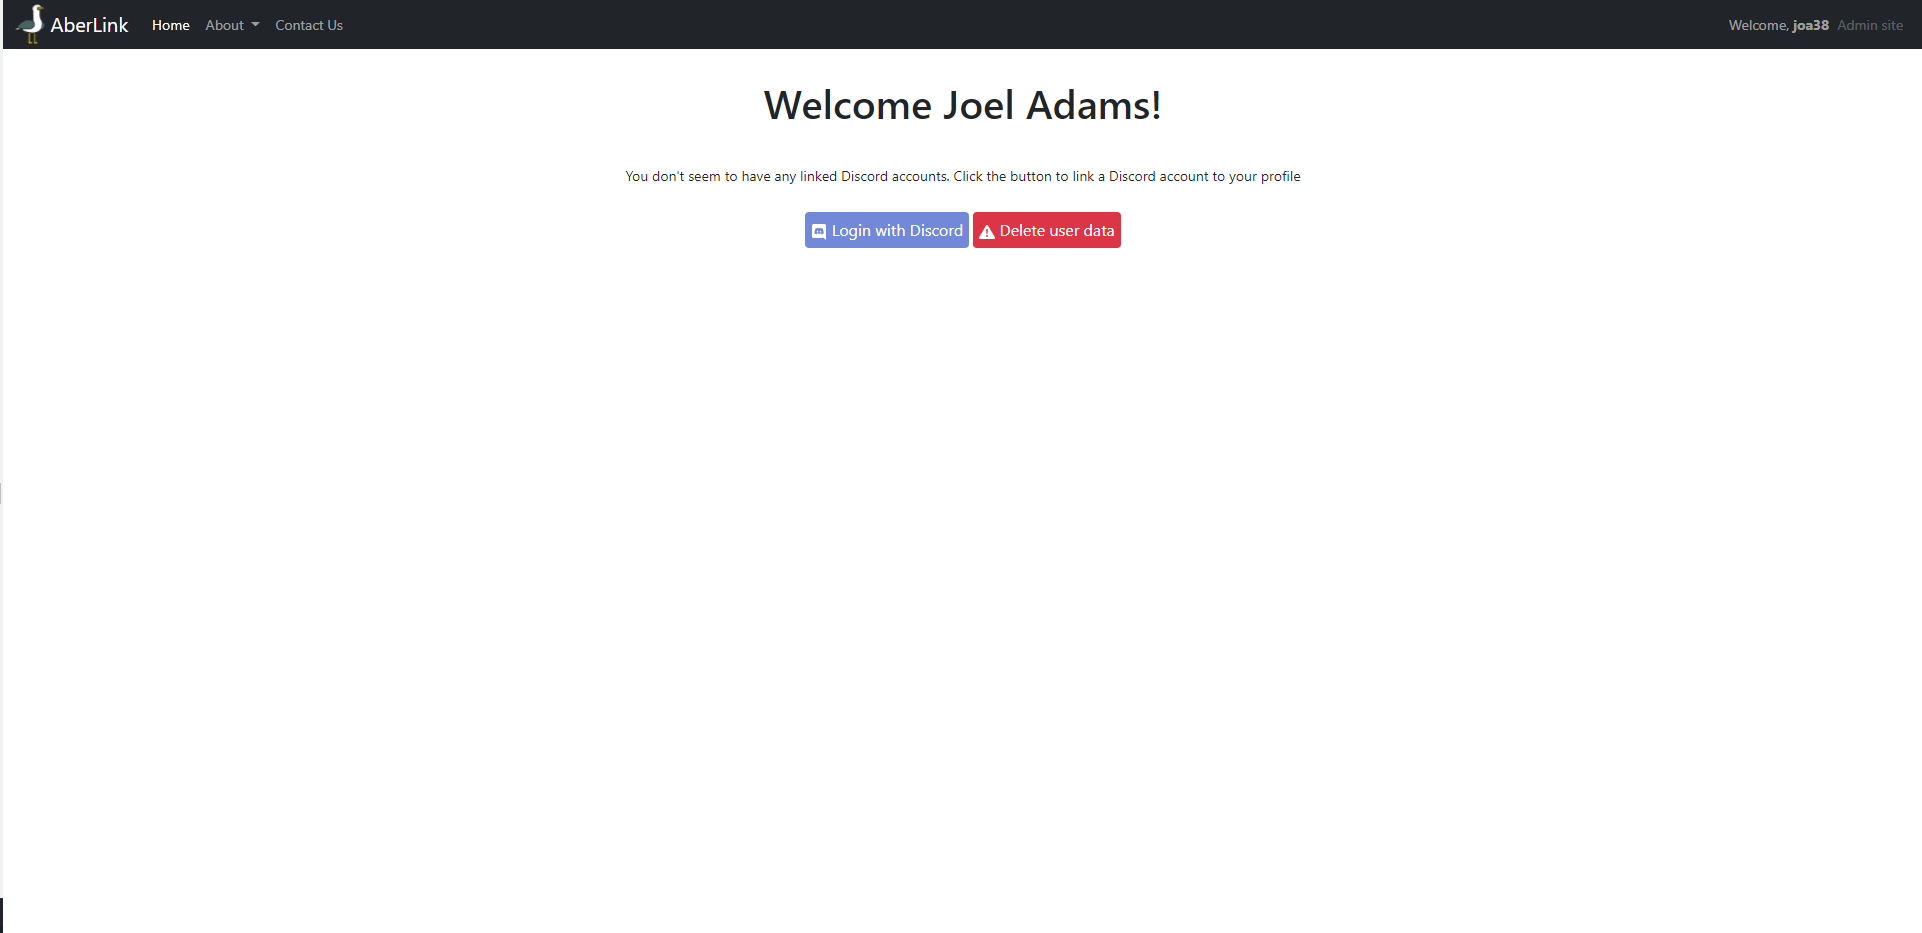
\includegraphics[width=1\linewidth]{Figures/website-acc-0.png}
	\caption{Final website with 0 linked Discord accounts}
	\label{fig:final-web-acc-0}
\end{figure}

\begin{figure}[H]
	\centering
	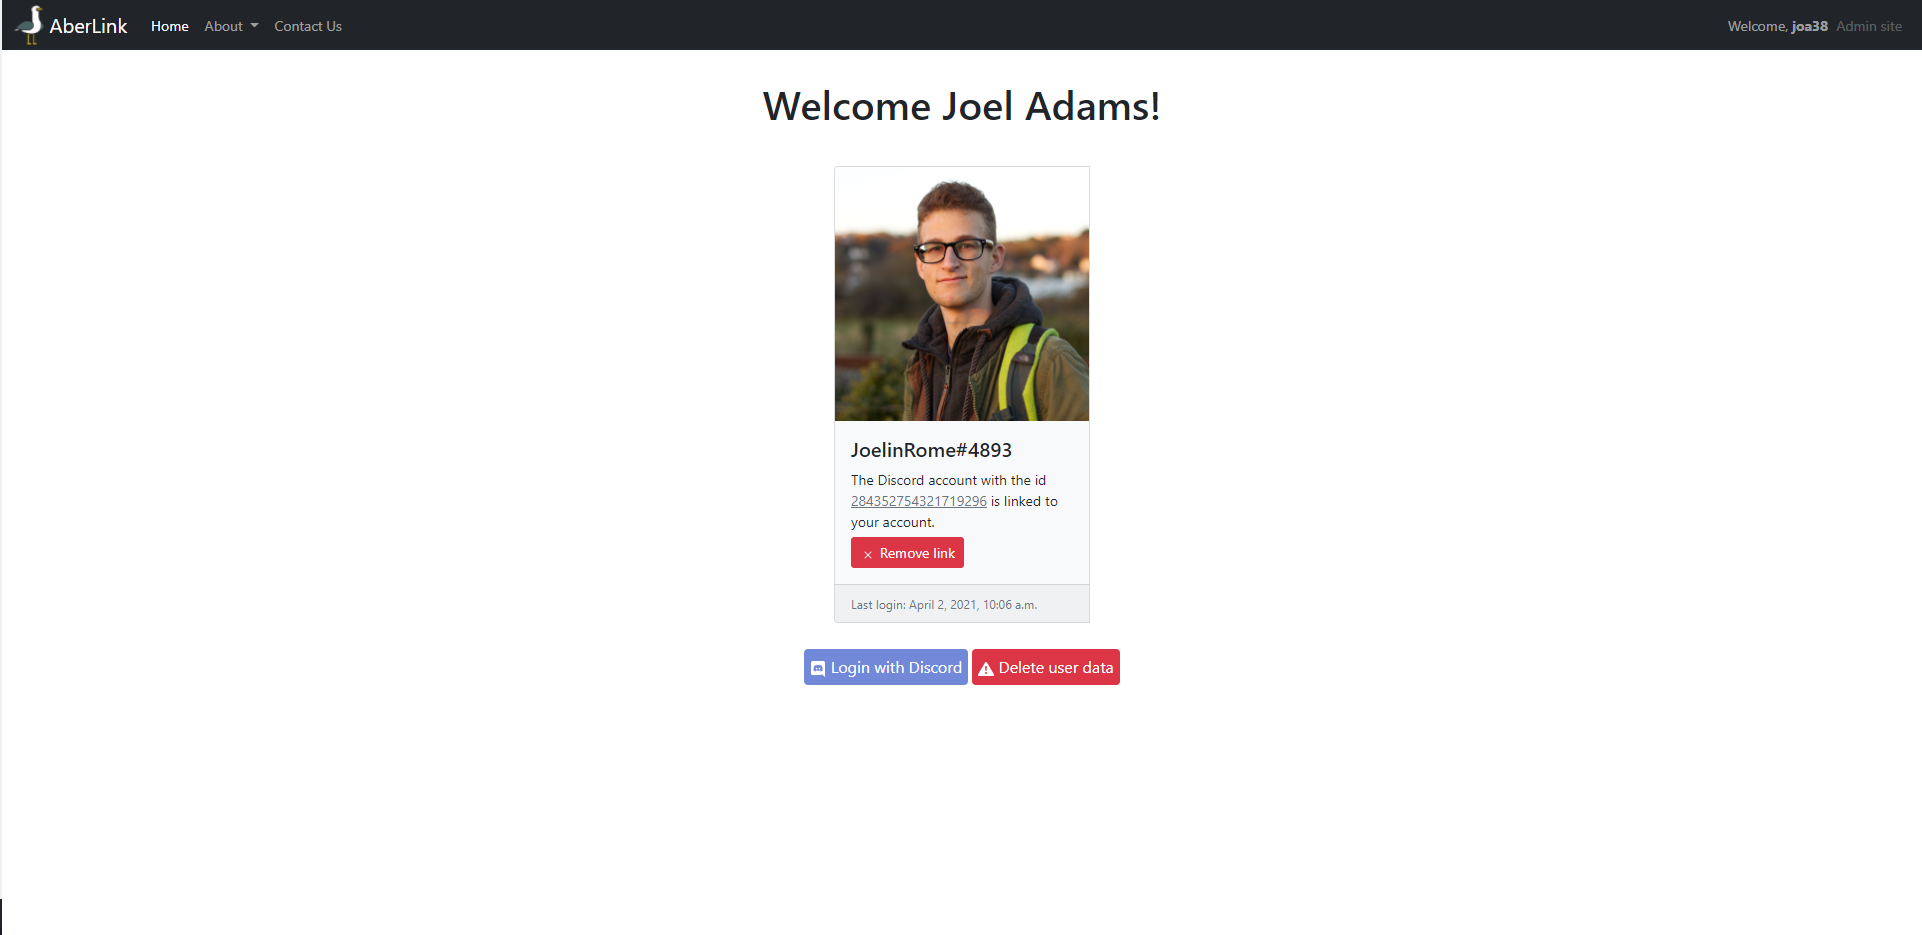
\includegraphics[width=1\linewidth]{Figures/website-acc-1.png}
	\caption{Final website with 1 linked Discord accounts}
	\label{fig:final-web-acc-1}
\end{figure}

\begin{figure}[H]
	\centering
	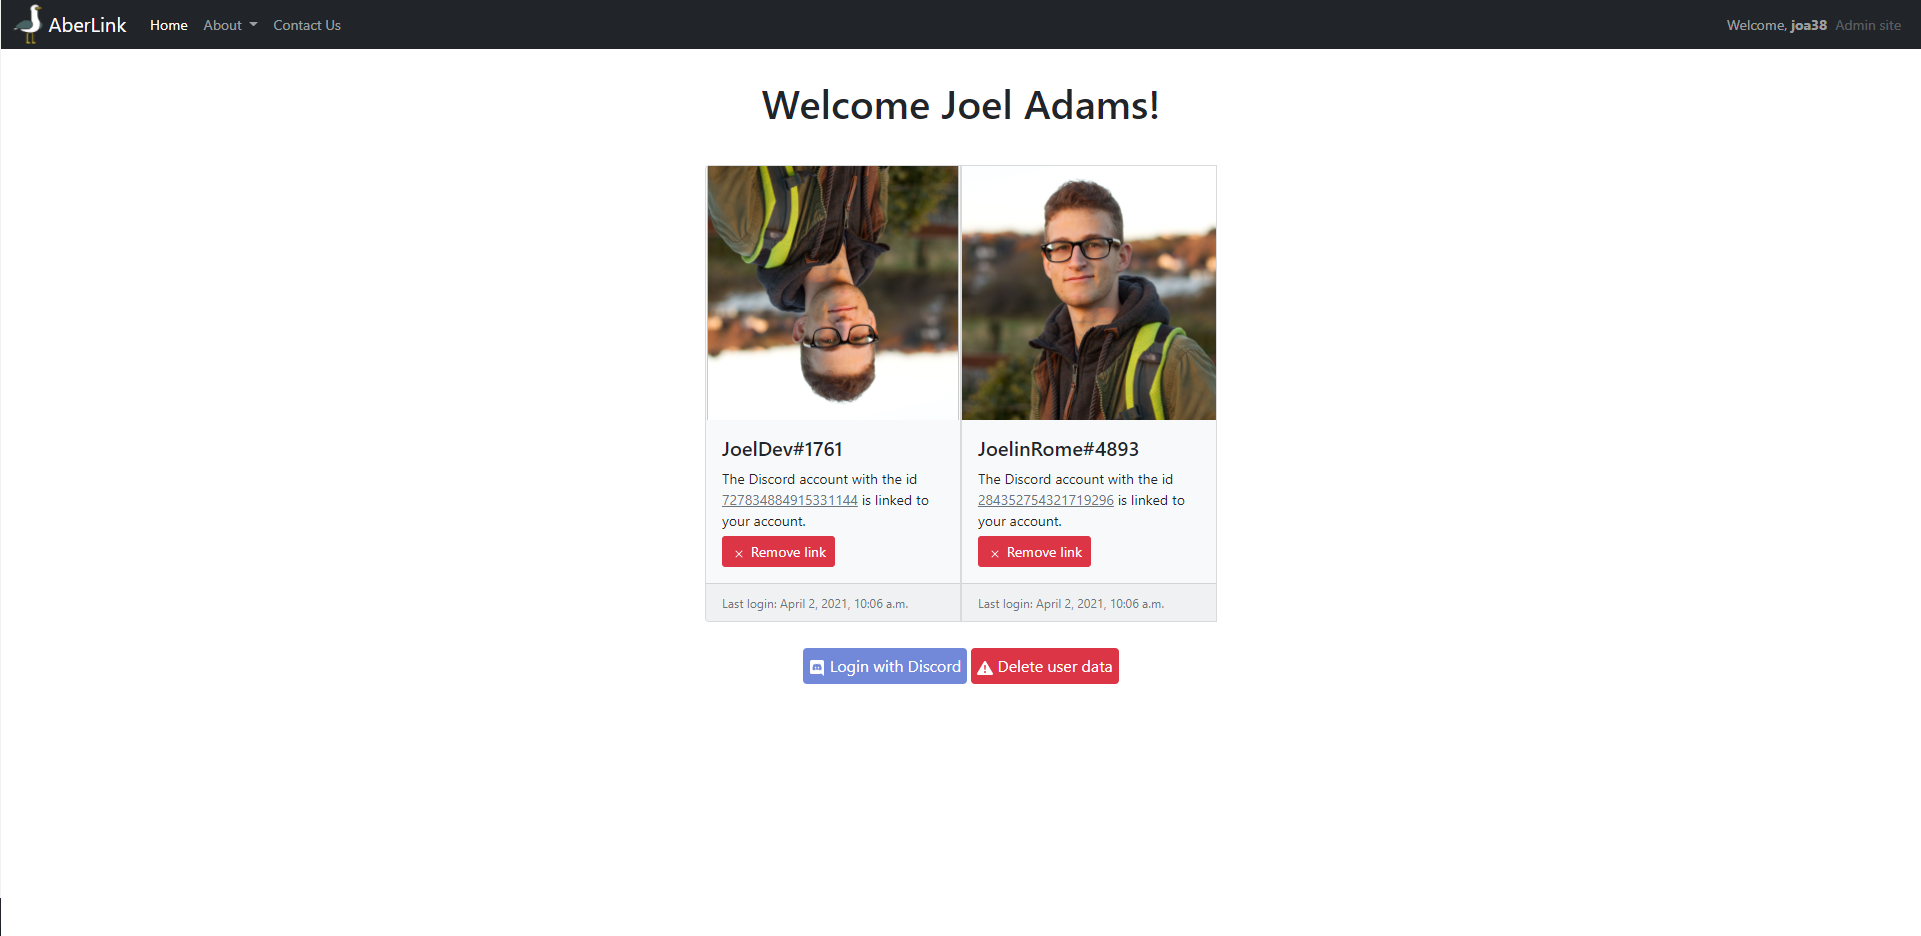
\includegraphics[width=1\linewidth]{Figures/website-acc-2.png}
	\caption{Final website with 2 linked Discord accounts}
	\label{fig:final-web-acc-2}
\end{figure}

\begin{figure}[H]
	\centering
	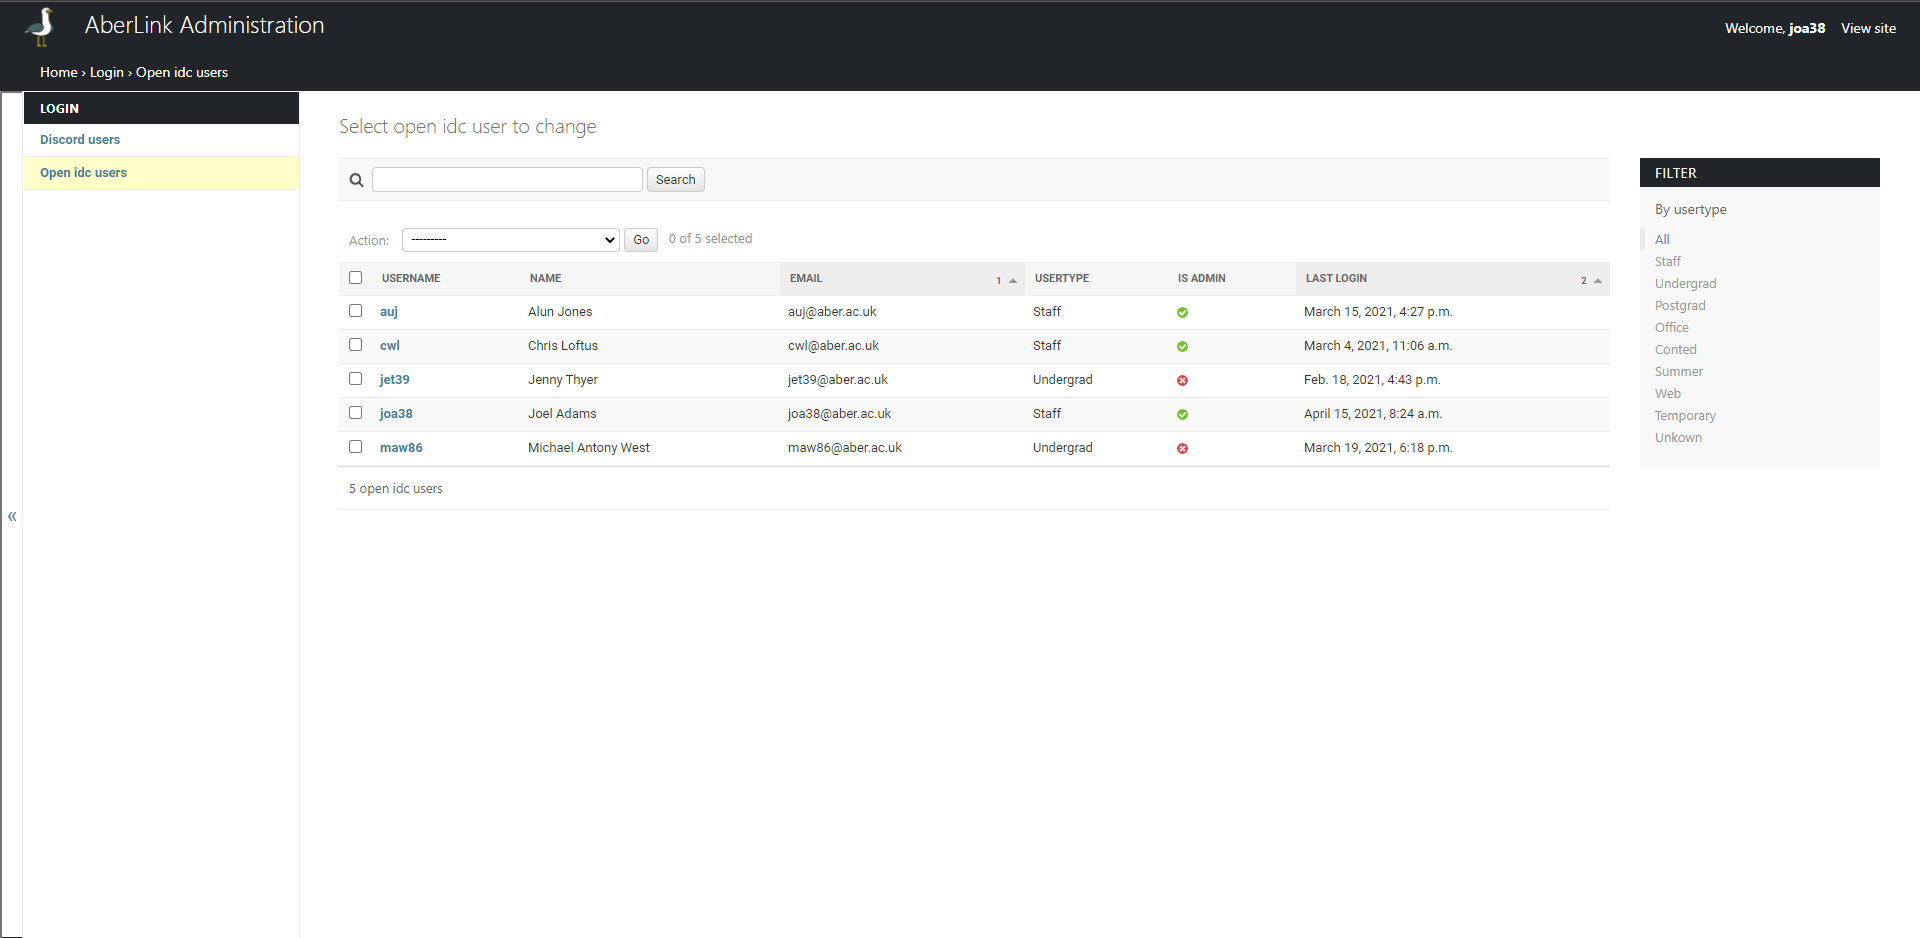
\includegraphics[width=1\linewidth]{Figures/website-admin-openidc.png}
	\caption{Final website Admin page for Aber accounts}
	\label{fig:final-web-admin-openidc}
\end{figure}

\begin{figure}[H]
	\centering
	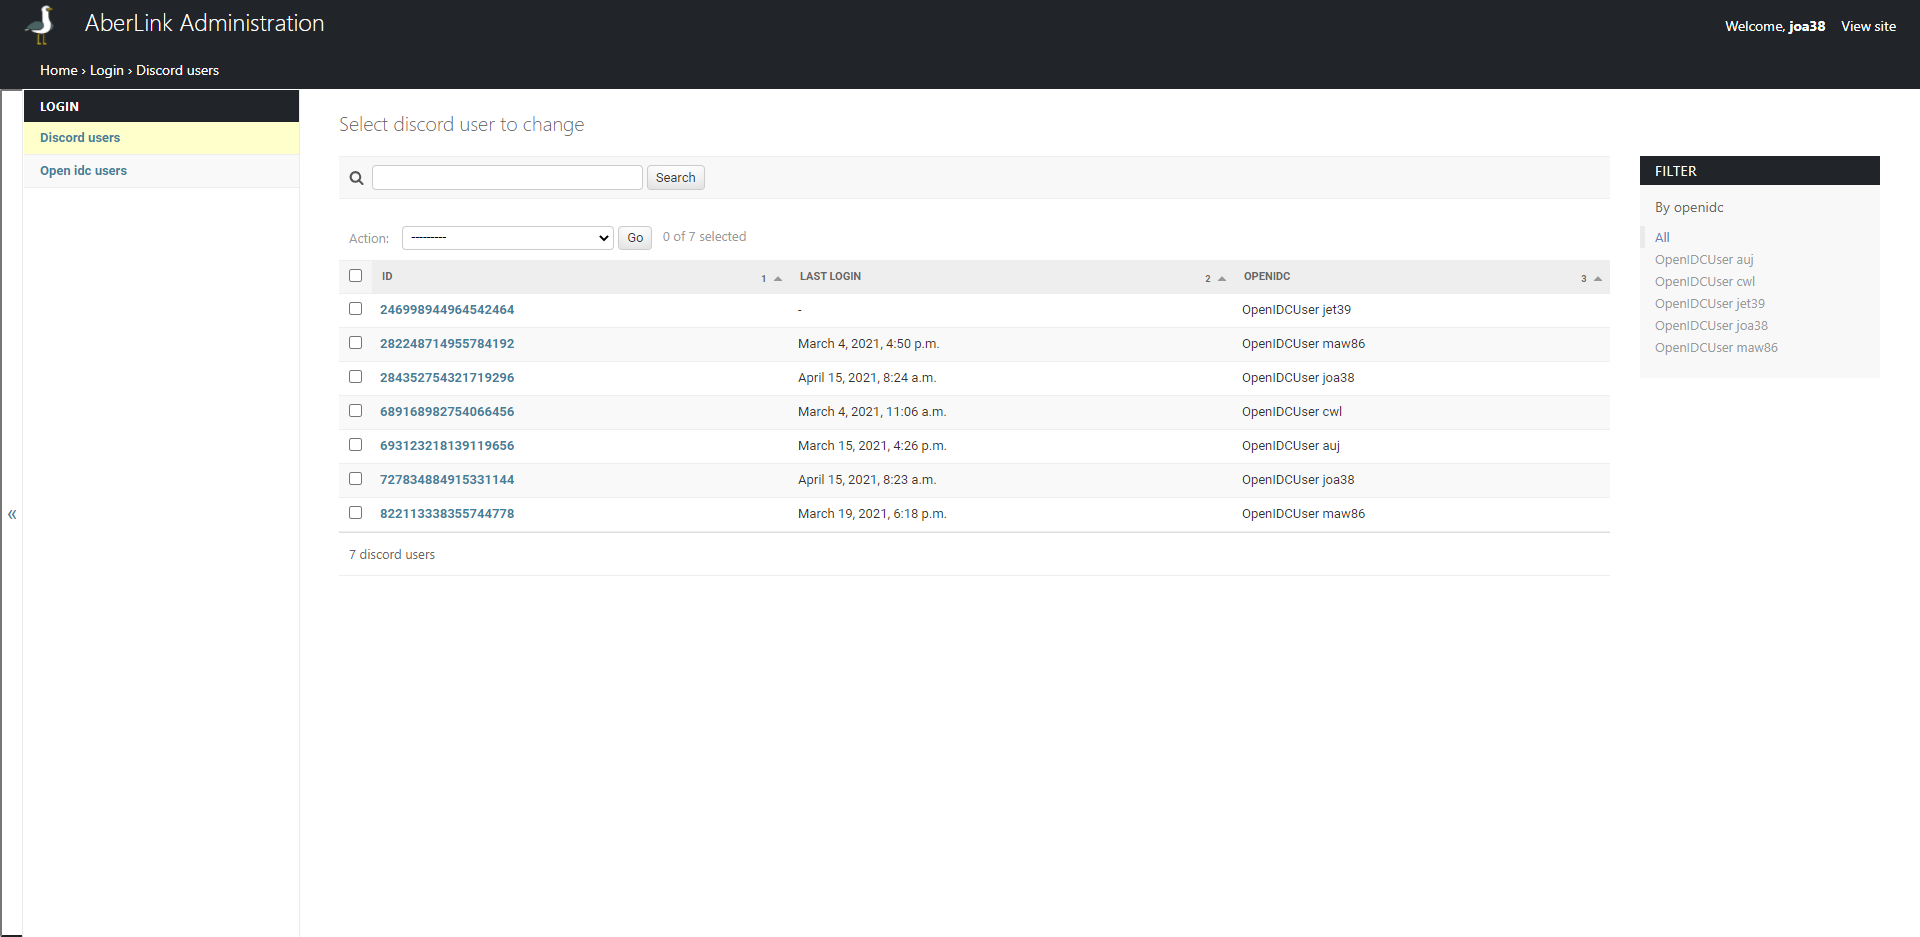
\includegraphics[width=1\linewidth]{Figures/website-admin-discord.png}
	\caption{Final website Admin page for Discord accounts}
	\label{fig:final-web-admin-dis}
\end{figure}

\subsection{Discord Bot}
The Discord bot (AberLink) implementation is exactly as described in the section \ref{sec2:discord} of the design. AberLink uses the Python library Discord.py \cite{discord.py} to make calls to and from the Discord API and to interact with the database it uses the Python library Psycopg2 \cite{psycopg2}. Both of these pieces of software are open-source and free to use in personal projects. 

\subsubsection{Setup and Configuration}
The bot contains a main file called AberLink.py that configures the bot giving it all the required permissions/settings to run. It loads the sensitive credentials from a .env file using the Python library dotenv \cite{dotenv}. This file contains key-value pairs that hold the Discord bot token that is accessible from the Discord developer portal \href{https://discord.com/developers/applications}{https://discord.com/developers/applications} and information required for the bot to connect to the database.

\begin{figure}[H]
	\begin{lstlisting}[language=Python]
# load the private discord token from .env file.
load_dotenv()
TOKEN = os.getenv('DISCORD_TOKEN')
WEBSITE = os.getenv('WEBSITE_URL')

# Initialise the database connection
PostgreSQL.connect()

# Initialise the Bot object with an accessible help Command object
helpCommand = DefaultHelpCommand()

bot = commands.Bot(
    command_prefix="!",
    help_command=helpCommand,
    intents=discord.Intents.all(),
)

bot.run(TOKEN)
\end{lstlisting}
\caption{Snippet of code from AberLink.py main Discord bot file}
\label{fig:discord-main-file}
\end{figure}

As seen in the figure above the key value pair for the \verb|DISCORD_TOKEN| is loaded in from the file and then used at the end of the code extract to run the bot. In the middle we see in important section called \verb|commands.Bot| that tells the bot key information such as which prefix to use that determines how a command is called. E.g. \verb|!| means that a command is invoked using \verb|!<command_name>|, by changing this then the command is invoked using that prefix. It is also not limited to a single character so can be \verb|AberLink| and then command would be invoked using \verb|AberLink<command_name>|.

\subsubsection{Discord Command Example}

The bot creates commands that can be used in a Discord server using the Discord.py \cite{discord.py} library. Below is an example of the ping command that is used as a way to check that the bot is alive. Discord.py turns this Python function into a Discord command when the decorator \verb|@commands.command(aliases=['p'])| is used where the \verb|aliases=['p']| parameter indicates an alias that can be used to call the command. The function then starts a timer using time() and stops after the first message is sent, then the message is edited to include the latency taken to edit and modify the message. Included in this response is also information on the database such as the latency, polling status and response time.

\begin{figure}[H]
\begin{lstlisting}[language=Python]
@commands.command(aliases=['p'])
async def ping(self, ctx: Context):
	"""
	Returns latency and response time of Discord and the database
	"""
	start_time = time()
	message = await ctx.send(f' pong `DWSP latency: {str(round(ctx.bot.latency * 1000))}ms`')
	end_time = time()
	db_latency = PostgreSQL.get_connection_latency()
	db_poll = PostgreSQL.get_polling_status()
	await message.edit(content=f' pong \n{emojis["discord"]} `DWSP latency: {str(round(ctx.bot.latency * 1000))}ms` ' +
    f'`Response time: {str(int((end_time - start_time) * 1000))}ms` \n' +
    f'{emojis["aberlink_database"]} `Database Polling status: {db_poll}` `Database latency: {db_latency}ms`')

\end{lstlisting}
\caption{Example of AberLink's ping command code}
\label{fig:discord-command-ping-code}
\end{figure}

The commands response is then sent to the Discord channel with a response that looks similar to the one pictured below.

\begin{figure}[H]
	\centering
	
\includegraphics[width=1\linewidth]{Figures/discord-ping-command.png}
	\caption{Example of ping command in Discord}
	\label{fig:discord-command-ping}
\end{figure}

\subsubsection{How do I access a list of the commands in AberLink?}
The Discord.py library contains a useful function called \verb|DefaultHelpCommand()| that will generate an automatic list of commands available in your program by analysing each function that has the command decorator \verb|@commands.command()|. The list of commands is then accessible through Discord using the command prefix plus the keyword help which in this case would be !help. Below is an example of the current output from the help command at time of this screenshot.  

\begin{figure}[H]
	\centering
	
\includegraphics[width=1\linewidth]{Figures/discord-help.png}
	\caption{Example of Discord help command to display list of Discord commands for AberLink}
	\label{fig:discord-help}
\end{figure}

\subsubsection{Error handling}
Discord.py includes a decorator called \verb|@Bot.event()| that goes inside of the AberLink.py file for dealing with bot events. This paired with a function called \verb|on_command_error()| deals with error messages. Below is an example of some of the if statements that deal with bot errors. The final else if command to check if the command is not found is extremely important as it tells the bot to ignore any commands that does not exist in the case where two Discord bots use the same command prefix but have different commands.

\begin{figure}[H]
\begin{lstlisting}[language=Python]
if isinstance(error, commands.errors.CheckFailure):
	await ctx.send(error)
elif isinstance(error, commands.errors.MissingRequiredArgument):
	await ctx.send('You are missing a required argument.')
elif isinstance(error, commands.errors.CommandNotFound):
	pass
\end{lstlisting}
\caption{Example of AberLink's on\_command\_error() checking statements}
\label{fig:discord-error-checking}
\end{figure}

\subsubsection{Server Configurations}
AberLink contains a feature called autoSetNickname that will automatically assign nicknames to users when they join or verify on the server by appending their aber username to the end of their name. e.g. JoelinRome\#4893 becomes JoelinRome [joa38]. This was added to help lecturers easily identify which student is which and if the student is uncomfortable with this they can always manually change it back. 

Some lecturers might not enjoy this feature and prefer to turn it off so included is a micro database using the python module \cite{shelve} that creates a file stored in the same directory as the Python file. This basically creates a file that can be accessed at any time and acts as persistent storage. It contains key value pairs e.g. \verb|{server_id : true}| that store a boolean on whether the automatic naming feature is enabled or disabled. 

\subsection{Database}\label{sec3:database}
The Database implementation was relatively straight forward as Django \cite{Django} generates all of the required tables for the project to function once you define the models. I've included the model used to generate OpenID Connect \cite{OpenID} aber user model below. In this figure you can see that there are two classes; OpenIDCUserManager to create a new database object and OpenIDCUser to make the database model. 

The OpenIDCUserManager class has three main parameters; one to call itself, a user which is a JSON object and password which is defaulted to None as no password data is stored. The information from the user object is passed throughout the code and is used to decide if the user should have admin permissions. The user is then saved to the database.

The OpenIDCUser class contains a nested class called usertypes that is a list of all the possible choices for incoming usertypes from user authentication. Further down we can see that there is a set of definitions for the database model such as the id, username, name, etc. Note however that the usertype definition uses the choices class to define what role a user may have. As this model is the main model used to authenticate users on the website Django requires that the model contains a few special items including a password which I have set to None and the arrays at the bottom called USERNAME\_FIELD and REQUIRED\_FIELDS.

\begin{figure}[H]
\begin{lstlisting}[language=Python]
class OpenIDCUserManager(BaseUserManager):
    def create_user(self, user, password=None):
        new_user = self.model(
            username = user['OIDC_CLAIM_preferred_username'],
            name = user['OIDC_CLAIM_name'],
            email = user['OIDC_CLAIM_email'],
            usertype = user['OIDC_CLAIM_usertype']
        )
        if user['OIDC_CLAIM_usertype'] == "staff":
            new_user.is_admin = True
        new_user.save(using=self._db)
        return new_user

class OpenIDCUser(AbstractBaseUser):
    objects = OpenIDCUserManager()

    class usertypes(models.TextChoices):
        STAFF = 'staff'
        UNDERGRAD = 'undergrad'
        POSTGRAD = 'postgrad'
        OFFICE = 'office'
        CONTED = 'conted'
        SUMMER = 'summer'
        WEB = 'web'
        TEMPORARY = 'temporary'
        UNKNOWN = 'unknown'

    id = models.AutoField(auto_created=True, primary_key=True, serialize=False)
    username = models.CharField(max_length=40)
    name = models.CharField(max_length=300)
    email = models.CharField(max_length=30)
    usertype = models.CharField(max_length=50, choices=usertypes.choices)
    last_login = models.DateTimeField(null=True)
    password = None
    is_active = models.BooleanField(default=True)
    is_admin = models.BooleanField(default=False)

    USERNAME_FIELD = 'id'
    REQUIRED_FIELDS = ['username', 'name', 'email', 'usertype']
\end{lstlisting}
\caption{Django database model of OpenID Connect Aber users}
\label{fig:django-database-code}
\end{figure}

The tables generated for the database are pictured below and they do differ quite drastically from the tables discussed during the design section \ref{sec2:database} of this document. This is because I was not originally accounting for the tables that get automatically generated by Django \cite{Django} that are required for the application to run. Below the figure is information to explain what the Django generated tables mean.

\begin{figure}[H]
	\centering
	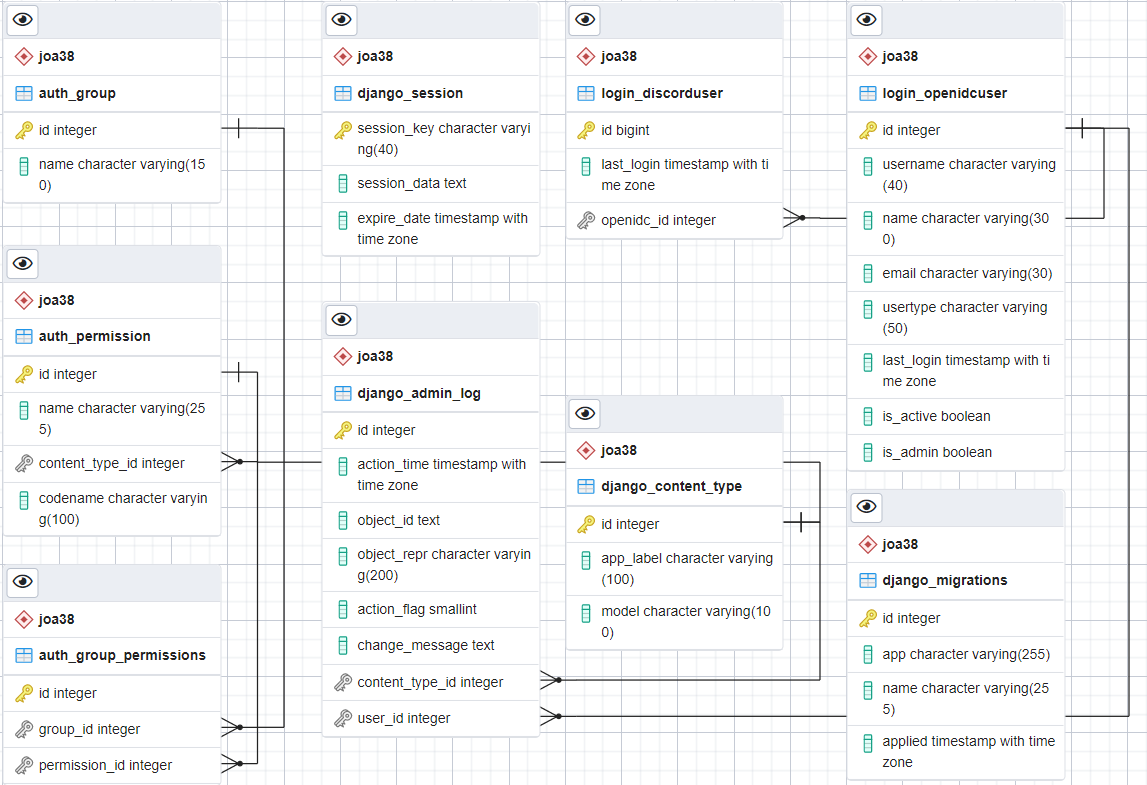
\includegraphics[width=1\linewidth]{Figures/er-diagram.png}
	\caption{Final Entity Relationship diagram for database}
	\label{fig:final-database}
\end{figure}

\begin{itemize}
	\item \textbf{User tables} - These two tables are the ones that have been discussed previously in this document for storing user data.
	\begin{itemize}
		\item \textbf{login\_openidcuser} - This table stores the OpenID Connect \cite{OpenID} information and is used as the authenticated user account.
		\item \textbf{login\_discorduser} - This table stores information on the discord user and contains a foreign key relationship with the table above.
	\end{itemize}
	\item \textbf{Django tables} - Tables generated by Django \cite{Django}
	\begin{itemize}
		\item \textbf{django\_migrations} - This table contains the history of the changes made to the database using Django. It acts as a way to revert to previous versions of the database in the case of 
		errors.
		\item \textbf{django\_session} - Stores sessions on the currently logged in users.
		\item \textbf{django\_content\_type} - Stores information on all available models in the database.
		\item \textbf{django\_admin\_log} - Stores history of logins for administrative users.
		\item \textbf{auth\_group \& auth\_group\_permissions \& auth\_permissions} - These tables are part of the backend for the authentication of users.
	\end{itemize}
\end{itemize}

Below are examples of the records that are stored in the database tables. 

\textbf{Note}: The column last\_login in the table \ref{tab:aber-table} contains the word datetime but should have a datetime object as seen in table \ref{tab:dis-table}. It has been removed so that the table fits nicely in this document.

\begin{table}[H]
	\centering
	\small
	\setlength\tabcolsep{2pt}
	\begin{tabular}{|c|c|c|c|c|c|c|c|}
		\hline
		\underline{id} & username & name & email & usertype & last\_login & is\_active & is\_admin \\
		\hline
		1 & joa38 & Joel Adams & joa38@aber.ac.uk & staff & datetime & t & t \\
		2 & jet39 & Jenny Thyer & jet39@aber.ac.uk & student & datetime & t & f \\
		3 & maw86 & Michael Antony West & maw86@aber.ac.uk & student & datetime & t & f \\
		\hline 
	\end{tabular}
	\caption{Aberystwyth user table example}
	\label{tab:aber-table}
\end{table}

\begin{table}[H]
	\centering
	\small
	\setlength\tabcolsep{2pt}
	\begin{tabular}{|c|c|c|}
		\hline
		\underline{id}                 & last\_login                   & openidc\_id* \\
		\hline
		727834884915331144 & 2021-02-18 16:43:47.067328+00 & 1           \\
		284352754321719296 & 2021-02-18 16:43:47.067328+00 & 1           \\
		246998944964542464 & 2021-02-04 11:14:40.057891+00 & 2           \\
		282248714955784192 & 2021-02-12 17:35:23.044226+00 & 3           \\
		\hline
	\end{tabular}
	\caption{Discord user table example}
	\label{tab:dis-table}
\end{table}

\section{Configuration and Setup}
After completion of this project there is a plan to setup this service permanently for the department so a folder was created called \textit{config} containing information on how to set up this project. This folder contains a README.md file that explains how and what is needed to be configured to get the system up and running properly. it also contains a bash script called setup.sh that installs and the relevant dependencies and sets up the virtual environments for the projects. Also included are a few example configuration files for Apache2 \cite{apache2}, Django \cite{Django}, OpenID Connect authentication \cite{OpenID} and Discord.py \cite{discord.py}.

\section{Unforeseen Issues}\label{sec3:unforeseen}
An issue that was encountered was with creating the custom user model in Django that would have been used to model the database. The documentation and videos found online about implementing user models were rather cryptic and difficult to understand, however after much research a video explaining how to implement a good custom user model was found that resolved the issues. Once this was completed I realised that Django is not happy with modelling the primary key of a table using a char so switched over to using an int. This turned out to be a good idea as Aberystwyth university tends to recycle old emails so over the next 5 years there could be an issue where the database would try and create a new entry in the database with the same email.
\begin{figure}[H]
	\centering
	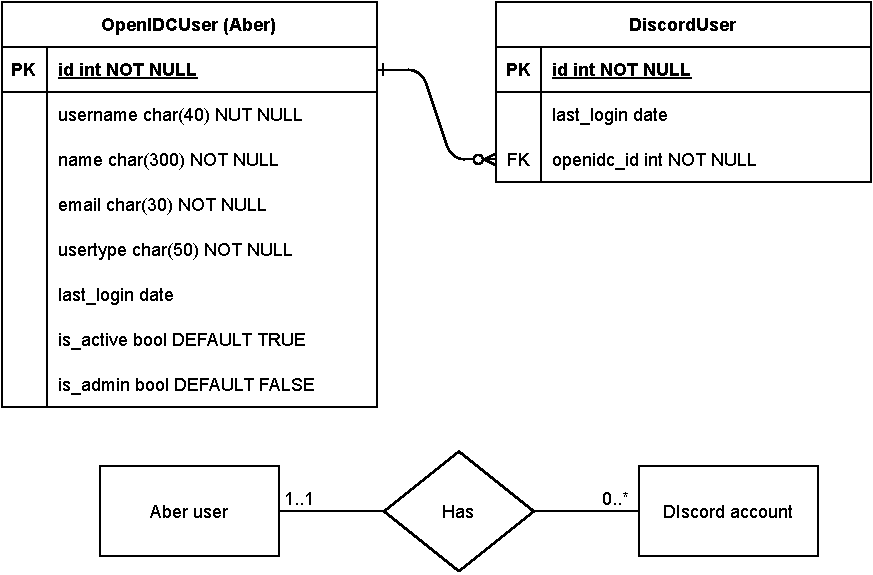
\includegraphics[width=0.8\linewidth]{Figures/database-er-1}
	\caption{Updated Entity relationship diagram for database}
	\label{fig:database-er-1}
\end{figure}

\section{Review}
\subsection{Review Against Planned Requirements}\label{sec3:pr}
Most of the planned requirements have not changed during implementation however some of the promised tasks have only been partially fulfilled. Please see Appendix \ref{tab:fr-test} for a table of the functional requirements specified in \ref{sec1:fr}. For more information on requirements that did not pass please see \ref{sec4:fr}.

In the final section of section \ref{sec1:obj} \textbf{Further potential work} I have decided against integrating DemoHelper into AberLink as this would greatly increase its complexity and make it much more difficult to maintain. Welsh language support has also not been implemented as I do not speak the language nor understand it well enough.

\subsection{Review Against Project Process}\label{sec3:pp}

Below is included a table describing the iterations and what was completed each one. These iterations were based on the list of objectives created in section \ref{sec1:obj} and span over the course of two months. For more detail please see the wordpress blog here \href{https://cs39440blog.wordpress.com/}{https://cs39440blog.wordpress.com/}.

\begin{longtable}[H]{| c | c | p{9cm} |}
\hline
Iteration & Time taken (days) & What happened? \\
\hline
1 & 5 & Research into services required to run the project and basic setup of uni container. Lots of meetings to discuss what data can be used/stored and began setup of API endpoint for attendance. \\
\hline
2 & 5 & Setup HTTPS on container, installed Django \cite{Django} and created basic website using it. Linked up Django to database and created basic Discord login system. \\
\hline
3 & 5 & Added OpenID Connect \cite{OpenID} to website for aber user login. Created basic models to link OpenID accounts to Discord accounts in PostgreSQL \cite{psql}. \\
\hline
4 & 7 & Created Admin pages and implemented proper database model for Discord and Aber users\\
\hline
5 & 5 & Created Discord bot skeleton and added support for it to connect to the database.\\
\hline
6 & 5 & Added attendance and verification to Discord bot. \\
\hline
7 & 5 & Added content to main webpage and option to delete a Discord account or all data. Added custom error message webpages for 400, 403, 404 and 500. \\
\hline
8 & 5 & Updated main user page so that it queries Discord API to get profile picture and username and update webpage with details. Added more features to Discord bot to interact with database.\\
\hline
9 & 5 & Created Configuration folder for installing the software along with bash script to install dependencies.\\
\hline
10 & 5 & Added Discord bot functionality to add configurations to a server and feature to automatically change Discord users nickname to append aber email.\\
\hline
11 & 16 & Working on LaTeX document for project report. \\
\hline
\caption{Project iterations and what occurred}
\label{tab:project-iterations}
\end{longtable}

Included is a graph of my GitLab commits over time below to help backup my table described above. 

\begin{figure}[H]
	\centering
	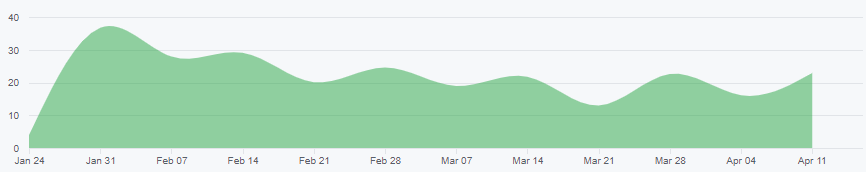
\includegraphics[width=1\linewidth]{Figures/gitlab-commit-graph.png}
	\caption{GitLab graph of commits over time}
	\label{fig:gitlab-graph}
\end{figure}
\chapter{Testing}

%Detailed descriptions of every test case are definitely not what is required here. What is important is to show that you adopted a sensible strategy that was, in principle, capable of testing the system adequately even if you did not have the time to test the system fully.

%Provide information in the body of your report and the appendix to explain the testing that has been performed. How does this testing address the requirements and design for the project?

%How comprehensive is the testing within the constraints of the project?  Are you testing the normal working behaviour? Are you testing the exceptional behaviour, e.g. error conditions? Are you testing security issues if they are relevant for your project? 

%Have you tested your system on ``real users''? For example, if your system is supposed to solve a problem for a business, then it would be appropriate to present your approach to involve the users in the testing process and to record the results that you obtained. Depending on the level of detail, it is likely that you would put any detailed results in an appendix.

%Whilst testing with ``real users'' can be useful, don't see it as a way to shortcut detailed testing of your own. Think about issues discussed in the lectures about until testing, integration testing, etc. User testing without sensible testing of your own is not a useful activity.

%The following sections indicate some areas you might include. Other sections may be more appropriate to your project.   

As previously mentioned in section \ref{sec1:pro} a Feature Driven Development (FDD) approach was used for this project, working in one week iteration windows to build and test the software. This included all of the testing sections mentioned below apart from automated testing which was completed at the end of the project instead.

The Discord.py Python framework does not contain any unit testing and there are no third party libraries which sufficiently perform this job. For the Django framework however there are some unit tests built in so they have been used in this project and are detailed further on in section \ref{sec4:unit-web}. These Django tests are used to cover both the website and the database as the website cannot be tested by itself. 

\section{Sample Data}
Sample data was considered for this project however it would be very difficult to implement because the OpenID Connect \cite{OpenID} system used to authenticate and log users in relies on a proper database to pull user data from. The University was not comfortable with creating and supplying fake user accounts that would authenticate with this system as the database where these would be used is currently live. This would mean that they could be stolen and used to access live systems such as Student Record or blackboard. The alternative to this would mean that a mock database would be needed which would take up a considerable work to create. The workaround for this system is far simpler and involved asking both staff and students to try out the system and test it until it breaks. The outcomes of this are detailed in section \ref{sec4:user-tesing}.

\section{Automated Testing}
Automated testing has been difficult for this project as mentioned above. Originally there was a plan to include automated testing by using the DevOps frameworks in Git, however as the universities GitLab instance was used then there was no access to dedicated pipelines/kubernite clusters to build and run the code.  

\subsection{Unit Tests}

\subsubsection{Website \& Database}\label{sec4:unit-web}
Django provides some useful documentation (\href{https://docs.djangoproject.com/en/3.1/topics/testing/}{https://docs.djangoproject.com/en/3.1/topics/testing/}) for creating unit tests for both Django and the database/user models. These tests are useful for checking that Discord accounts and OpenID Connect \cite{OpenID} Aber accounts link up properly and that webpage urls are correct and render the appropriate content. All of the following tests can be found in the file located in this path \verb|src\AberLinkAuthentication\login\tests.py|. 

Below are two testing classes; one called TestUrls and one called TestModels. These are responsible for testing that the urls are correctly found and that adding new users to the database works as intended. Included below is an example of each test:

\begin{figure}[H]
\begin{lstlisting}[language=Python]
def test_url_discord_redirect(self):
    url = reverse('Discord-response')
    self.assertEquals(resolve(url).func, views.discord_oauth2_redirect)
\end{lstlisting}
\caption{Django URL render test}
\label{fig:django-url}
\end{figure}
As seen above the test function simply gets the name of the url `Discord-response' and then checks that it returns the correct Python function (view) to render that page

\begin{figure}[H]
\begin{lstlisting}[language=Python]
def test_model_openidc_user_staff(self):
    self.openidc_user2 = OpenIDCUser.objects.create(
        username="abc123",
        name="Bob Ross",
        email="abc123@aber.ac.uk",
        usertype="staff"
    )
    self.assertEquals(self.openidc_user2.username, "abc123")
    self.assertEquals(self.openidc_user2.name, "Bob Ross")
    self.assertEquals(self.openidc_user2.email, 
    "abc123@aber.ac.uk")
    self.assertEquals(self.openidc_user2.usertype, "staff")
    self.assertEquals(self.openidc_user2.is_admin, True)
\end{lstlisting}
\caption{Django database render test}
\label{fig:django-database}
\end{figure}
This function creates a new user object and then checks to make sure that the user has been given the admin and has the usertype of staff.

\subsubsection{Discord}
Unit testing in Discord.py is impossible as there is no included framework for it and there are no external libraries capable of testing to check that it works.

\subsection{Stress Testing}
To test the websites capacity to deal with 100s of requests ApacheBenchmark \cite{apacheBenchmark} is used which is a built into the Apache2 \cite{apache2} and is a module used to request a webpage and measure response time. To test this the OpenID Connect \cite{OpenID} authentication system  was temporarily disabled so that HTML gets served to the incoming requests instead of being redirected to the login page. Due to the nature of the websites implementation you cannot query the main page because the user is not authenticated and the page cannot display information on the user, however it can query one of the subpages that does not require authentication. The following line of code was used to complete the request with 1000 requests and 100 concurrent threads to attempt to tank the website's performance.

\verb|ab -n 1000 -c 100 https://mmp-joa38.dcs.aber.ac.uk/privacy-policy|

This command generates the following report which shows that the website is capable at easily handling this many requests simultaneously. The longest response time for serving the requests was 642ms which is still adequately fast for the average user and shows that Django handles requests reasonable well. It can also serve on average 174 requests per second and I expect that the website will never be receiving more that 300 requests at the exact same time which can definitely be handled as seen from these results. Another factor to consider is that this development build is currently running on a small container that only has access to a small amount of resources whereas in the final build it will have access to far more resources so could serve requests up even quicker.

%\begin{figure}[hbt!]
\begin{verbatim}
Server Software:        Apache/2.4.38
Server Hostname:        mmp-joa38.dcs.aber.ac.uk
Server Port:            443
SSL/TLS Protocol:       TLSv1.2,ECDHE-RSA-AES256-GCM-SHA384,2048,256
Server Temp Key:        X25519 253 bits
TLS Server Name:        mmp-joa38.dcs.aber.ac.uk

Document Path:          /privacy-policy
Document Length:        12448 bytes

Concurrency Level:      100
Time taken for tests:   5.719 seconds
Complete requests:      1000
Failed requests:        0
Total transferred:      12734000 bytes
HTML transferred:       12448000 bytes
Requests per second:    174.86 [#/sec] (mean)
Time per request:       571.882 [ms] (mean)
Time per request:       5.719 [ms] (mean, across all concurrent requests)
Transfer rate:          2174.50 [Kbytes/sec] received

Connection Times (ms)
              min  mean[+/-sd] median   max
Connect:        9  422 105.1    458     547
Processing:     7   86  61.1     67     404
Waiting:        6   83  60.1     64     381
Total:         42  508  96.3    531     642

Percentage of the requests served within a certain time (ms)
  50%    531
  66%    550
  75%    560
  80%    565
  90%    574
  95%    583
  98%    593
  99%    602
 100%    642 (longest request)
\end{verbatim}
%\caption{Output from running Apache Benchmark on the website}
%\label{fig:ab}
%\end{figure}

\section{User Interface Testing}
Testing the user interface for the AberLink is mostly straight forward as Discord has full control over the UI so I have had no testing to do on that front.

The UI of the website uses the library Bootstrap \cite{bootstrap} as it is built from the ground up with responsive design in mind and saves a lot of time that would be required to re-learn CSS fully. This meant that website would scale very nicely and uniformly depending on screen size. To ensure that the website scales and performs well the website and all of its content have been tested on multiple devices. It has been tested on mobile devices, iPads and laptops with screens ranging from 11in to 40in using Safari, Chrome, Edge and Firefox. The website has also been tested on HTML the validation website \href{https://validator.w3.org/}{https://validator.w3.org/} to ensure that there are no large errors that may cause the website to not load on certain machines.

\section{User Testing}\label{sec4:user-tesing}
Throughout this project I have worked with the mindset that you develop small sections of code and then review what effect they have on the system. This helps to catch errors as it is much easier to backtrack through small sections of code.

For user testing I asked in the comp sci server if students could try and login to the website and break it. This turned out to work very well and helped to find a few edge cases that I had previously missed in the code.

\subsection{Attendance API Endpoint Testing}
The supplied API for attendance has been tested using user testing and the University provided me with 3 different endpoints to test. They are listed below along their responses.

\begin{verbatim}
https://integration.aber.ac.uk/joa38/good.php
{"status_updated":"true","request":"200","module_code":"CS32120"}    
\end{verbatim}

\begin{verbatim}
https://integration.aber.ac.uk/joa38/bad.php
{"status_updated":"false","request":"400",
"error_message":"Unknown user or no event"}
\end{verbatim}

\begin{verbatim}
https://integration.aber.ac.uk/joa38/submit.php
Actual live endpoint. Returns either of the two JSON messages 
above along with the corrected module_code
\end{verbatim}

\section{Functional Requirements}\label{sec4:fr}
The final testing was conducted using a list of functional requirements set out in section \ref{sec1:fr} and the testing table can be found in Appendix \ref{tab:fr-test}. Most of the tests passed correctly however some of them have not.

The Functional requirements FR3.4 \& FR4.7 have only been partially fulfilled. This was a purposeful design choice as it would mean that the website would require that Discord servers are added to database and that they would have to be updated when any issues occurred. This was also bad because this list would have to be maintained and could not be automatically updated which would lead to it breaking down the line.
\chapter{Evaluation}

% Examiners expect to find a section addressing questions such as:

% \begin{itemize} 
%    \item Were the requirements correctly identified? 
%    \item Were the design decisions correct?
%    \item Could a more suitable set of tools have been chosen?
%    \item How well did the software meet the needs of those who were expecting to use it?
%    \item How well were any other project aims achieved?
%    \item If you were starting again, what would you do differently?
% \end{itemize}

% Other questions can be addressed as appropriate for a project. 

% The questions are an indication of issues you should consider. They are not intended as a specification of a list of sections.

% The evaluation is regarded as an important part of the project report; it should demonstrate that you are capable not only of carrying out a piece of work but also of thinking critically about how you did it and how you might have done it better. This is seen as an important part of an honours degree. 

% There will be good things in the work and aspects of the work that could be improved. As you write this section, identify and discuss the parts of the work that went well and also consider ways in which the work could be improved. 

% In the latter stages of the module, we will discuss the evaluation. That will probably be around week 9, although that differs each year. 

\section{Were the requirements correctly identified?}
I believe that the requirements for this project have been correctly identified and have fit the scope well, however, as previously explained in section \ref{sec4:fr} the scope of the project was reduced slightly. The rest of the requirements were achieved to their fullest.

\section{Were the design decisions correct?}
Most of the design decisions were correct, however, as detailed in section \ref{sec3:database} I did not account for Django creating its own tables used for running the website. 

I also did not know that Django is unhappy with using non-numerical primary keys hence my original table design in section \ref{sec2:database} failed and I had to use automatically generated numbers for the primary key of the Aber users account table as seen in section \ref{sec3:unforeseen}.

\section{Could a more suitable set of tools have been chosen?}
I believe that my choice of software tools was very good for this project and very manageable. I believe that if I attempted this project again I would attempt to try building up the website using a tool like React or Node.js instead of Django. These tools would give me more versatility and allow me to experiment further with the website but would be considerably harder to work with. I can however see one pitfall which is that the administration pages created by Django by default would have to be built from the ground up in JavaScript.

I would also have used a different authentication system such as the office 365 authentication system as it can be used in a much less invasive way and allows users to browse the websites content without logging in. The OpenID Connect system relied on the whole website requiring authentication which was annoying as it gave me little flexibility on what could be done. By using the office 365 login I could have also gained access to profile pictures which would have made a nice addition for the website.

\section{How well did the software meet the needs of those who were expecting to use it?}
As seen in section \ref{sec4:user-tesing} of user testing most users were very happy with the service as a whole. Wherever improvement was suggested I have attempted to increase the experience.

\section{Time Management of the project}
The project was managed very well and I completed to coding of the project well in advance so had lots of time to tidy up the project and add new quality of life features. Please see section \ref{sec3:pp} for more information on project iterations.

\section{Project Meetings and Blog}
Project meetings usually occurred once a week and alternated between group meetings and individual meetings. The individual meetings were really helpful as they acted as a reason for me to have a working example available for each meeting. I also had a few other meetings with other members of staff from the University to discuss what could be used in the project and policies that I had to follow. 

The project blog was updated roughly once a week however during the earlier sections of the project it was updated once every few days due to a higher amount of work being performed. The blog can be found here \href{https://cs39440blog.wordpress.com/}{https://cs39440blog.wordpress.com/}.

%TC:ignore
\setemptyheader

\nocite{*} % include everything from the bibliography, irrespective of whether it has been referenced.

\addcontentsline{toc}{chapter}{Annotated Bibliography} % Adds References to contents page

\bibliographystyle{StylesAndReferences/IEEEannotU}
\renewcommand{\bibname}{Annotated Bibliography} 

\bibliography{StylesAndReferences/references} % References file


\setemptyheader

\addcontentsline{toc}{chapter}{Appendices}
\chapter*{Appendices}
% The appendices are for additional content that is useful to support the discussion in the report. It is material that is not necessarily needed in the body of the report, but its inclusion in the appendices makes it easy to access. 

% For example, if you have developed a Design Specification document as part of a plan-driven approach for the project, then it would be appropriate to include that document as an appendix. In the body of your report you would highlight the most interesting aspects of the design, referring your reader to the full specification for further detail.

% If you have taken an agile approach to developing the project, then you may be less likely to have developed a full requirements specification. Perhaps you use stories to keep track of the functionality and the 'future conversations'. It might not be relevant to include all of those in the body of your report. Instead, you might include those in an appendix. 

% There is a balance to be struck between what is relevant to include in the body of your report and whether additional supporting evidence is appropriate in the appendices. Speak to your supervisor or the module coordinator if you have questions about this.
\pagebreak

% start the appendix - sets up different numbering
\fancypagestyle{plain}{%
%\fancyhf{} % clear all header and footer fields
\fancyhead[L]{Appendix\ \thechapter}
\fancyhead[R]{\leftmark}}

\appendix
\fancyhead[L]{Appendix\ \thechapter}
\fancyhead[R]{\leftmark}
\fancyhead[C]{}
\fancyfoot[C]{\thepage}
\renewcommand{\headrulewidth}{0.4pt}
\renewcommand{\chaptermark}[1]{\markboth{#1}{}}

\fancyhead[L]{Appendix\ \thechapter}
\fancyhead[R]{\leftmark}
\fancyfoot[C]{{\thepage} of \pageref{LastPage}}

% include any appendices here
\chapter{Third-Party Code and Libraries}

% If you have made use of any third party code or software libraries, i.e. any code that you have not designed and written yourself, then you must include this appendix. 

% As has been said in lectures, it is acceptable and likely that you will make use of third-party code and software libraries. If third party code or libraries are used, your work will build on that to produce notable new work. The key requirement is that we understand what your original work is and what work is based on that of other people. 

% Therefore, you need to clearly state what you have used and where the original material can be found. Also, if you have made any changes to the original versions, you must explain what you have changed. 

% The following is an example of what you might say. 

% Apache POI library - The project has been used to read and write Microsoft Excel files (XLS) as part of the interaction with the client's existing system for processing data. Version 3.10-FINAL was used. The library is open source and it is available from the Apache Software Foundation 
% \cite{apache_poi}. The library is released using the Apache License 
% \cite{apache_license}. This library was used without modification. 

% Include as many declarations as appropriate for your work. The specific wording is less important than the fact that you are declaring the relevant work.
I declare that all the following libraries are unmondified.

\begin{itemize}
    \item \textbf{Pipenv} \cite{pipenv} - This is a Python package manager that is used throughout this project to create and maintain virtual environments. It uses Pipfiles (text files) to store a list of dependencies that are then downloaded and stored in a virtual environment. In this project I have two Pipfiles; one for the website (\verb|src\AberLinkAuthentication|) and one for the Discord bot (\verb|src\AberLinkDiscord|). This library uses the MIT license so is free to use.
    \item \textbf{Django} \cite{Django} - This is a Python web framework used for building websites. It is used to display the webpages, sign users in and help users and staff manage their data. This library is open source and provided by the \href{https://www.djangoproject.com/trademarks/#:~:text=Django%20is%20an%20Open%20Source,the%20use%20of%20a%20trademark.}{Django Software Foundation}.
    \item \textbf{Apache2} \cite{apache2} - This Debian \cite{debian} package is responsible for hosting a HTTP web server. In this case it hosts the Django \cite{Django} framework so it can be accessed on the web. This library is released under the \href{https://www.apache.org/licenses/LICENSE-2.0}{Apache License, Version 2.0}.
    \item \textbf{libapache2-mod-auth-openidc} \cite{libapache2-mod-auth-openidc} - Debian \cite{debian} package used to authenticate users when they first connect to the site. It authenticates users against their Aberystwyth University account and then creates a session where they can access content on the website. This library is released under the \href{https://static.fsf.org/nosvn/directory/fdl-1.3-standalone.html}{GNU Free Documentation License}
    \item \textbf{certbot} \cite{certbot} - This package was only briefly required to setup HTTPS on the website using Let's Encrypt \cite{letsencrypt}. Once SSL certificates have been made cerbot then runs a cronjob in the background to update it. This library is licensed under the \href{https://certbot.eff.org/faq#what-are-the-licenses-for-certbot-and-this-website}{Apache 2.0 license}
    \item \textbf{psycopg2} \cite{psycopg2} - This library is used for talking to PostgreSQL databases in Python. The version used here is called psycopg2-binary and it requires two additional dependencies to be built libpq-dev \cite{libpq-dev} and python-dev \cite{python-dev}. This library is licensed under the \href{https://www.psycopg.org/license/}{GNU Lesser General Public License}.
    \item \textbf{Discord.py} \cite{discord.py} - This Python library is used to create and write the Discord bot. It is basically an interface that allows me to write bots without making API requests straight to Discord. This library is licensed under the \href{https://github.com/Rapptz/discord.py/blob/master/LICENSE}{MIT License}.
    \item \textbf{Requests} \cite{requests} - It is used to make HTTP requests to the web. In this project it is used in the website to get information from the Discord login and in the Discord bot it is used to send and receive data from the attendance API endpoint \href{https://integration.aber.ac.uk/joa38/submit.php}{https://integration.aber.ac.uk/joa38/submit.php}. This library is licensed under the \href{https://pypi.org/project/requests/}{Apache Software License (Apache 2.0)}
    \item \textbf{Pytz, SQLParse \& ASGIref} \cite{pytz} \cite{sqlparse} \cite{asgiref} - These are dependencies required to work with Django. pytz helps with managing timezones and timezone data. SQLParse handles SQL queries, formatting and splitting. Asgiref is an interface used to talk between Apache2 \cite{apache2} and Django \cite{Django} for web server hosting and frameworks. These libraries are all licensed under the MIT License.
\end{itemize}
\chapter{Ethics Submission}

This appendix includes a copy of the ethics submission for the project. After you have completed your Ethics submission, you will receive a PDF with a summary of the comments. That document should be embedded in this report, either as images, an embedded PDF or as copied text. The content should also include the Ethics Application Number that you receive. 
%\chapter{Code Examples}

For some projects, it might be relevant to include some code extracts in an appendix. You are not expected to put all of your code here - the correct place for all of your code is in the technical submission that is made in addition to the Project Report. However, if there are some notable aspects of the code that you discuss, including that in an appendix might be useful to make it easier for your readers to access. 

As a general guide, if you are discussing short extracts of code then you are advised to include such code in the body of the report. If there is a longer extract that is relevant, then you might include it as shown in the following section. 

Only include code in the appendix if that code is discussed and referred to in the body of the report. 

\section{Random Number Generator}

The Bayes Durham Shuffle ensures that the psuedo random numbers used in the simulation are further shuffled, ensuring minimal correlation between subsequent random outputs \cite{NumericalRecipes}.

\begin{verbatim}
 #define IM1 2147483563
 #define IM2 2147483399
 #define AM (1.0/IM1)
 #define IMM1 (IM1-1)
 #define IA1 40014
 #define IA2 40692 
 #define IQ1 53668
 #define IQ2 52774
 #define IR1 12211
 #define IR2 3791
 #define NTAB 32
 #define NDIV (1+IMM1/NTAB)
 #define EPS 1.2e-7
 #define RNMX (1.0 - EPS)
 
 double ran2(long *idum)
 {
   /*---------------------------------------------------*/
   /* Minimum Standard Random Number Generator          */
   /* Taken from Numerical recipies in C                */
   /* Based on Park and Miller with Bays Durham Shuffle */
   /* Coupled Schrage methods for extra periodicity     */
   /* Always call with negative number to initialise    */
   /*---------------------------------------------------*/	
 
   int j;
   long k;
   static long idum2=123456789;
   static long iy=0;
   static long iv[NTAB];
   double temp;
 
   if (*idum <=0)
   {
     if (-(*idum) < 1)
     {
       *idum = 1;
     }else
     {
       *idum = -(*idum);
     }
     idum2=(*idum);
     for (j=NTAB+7;j>=0;j--)
     {
       k = (*idum)/IQ1;
       *idum = IA1 *(*idum-k*IQ1) - IR1*k;
       if (*idum < 0)
       {
         *idum += IM1;
       }
       if (j < NTAB)
       {
         iv[j] = *idum;
       }
     }
     iy = iv[0];	
   }
   k = (*idum)/IQ1;
   *idum = IA1*(*idum-k*IQ1) - IR1*k;
   if (*idum < 0)
   {
     *idum += IM1;
   }
   k = (idum2)/IQ2;
   idum2 = IA2*(idum2-k*IQ2) - IR2*k;
   if (idum2 < 0)
   {
     idum2 += IM2;
   }
   j = iy/NDIV;
   iy=iv[j] - idum2;
   iv[j] = *idum;
   if (iy < 1)
   {
     iy += IMM1;
   }
   if ((temp=AM*iy) > RNMX)
   {
     return RNMX;
   }else
   {
     return temp;	
   }
 }
 
\end{verbatim}


\chapter{Functional Requirements Table}

%\begin{table}[H]
\begin{longtable}{| c | c | p{10cm} |}
\hline
Functional Requirement & Passed? & How? \\
\hline
FR1 & \color{ForestGreen}Yes & Passed all requirements. Using functions from file \textit{AberLinkAuthentication/login/views.py}\\
\hline
FR1.1 & \color{ForestGreen}Yes &  OpenID Connect only authenticates aber users.\\
\hline
FR1.2 & \color{ForestGreen}Yes & function \textit{openidc\_response()} gets metadata from OpenID Connect login and usertype.\\
\hline
FR1.3 & \color{ForestGreen}Yes & \textit{openidc\_response()} gets user information and logs user in or creates a new account with the correct privileges.\\
\hline
FR2 & \color{ForestGreen}Yes & Passed all requirements. Using functions from file \textit{AberLinkAuthentication/login/views.py}\\
\hline
FR2.1 & \color{ForestGreen}Yes & \textit{discord\_oauth2\_redirect()} gets metadata by getting authorization from url code and calls \textit{exchange\_code()} to query Discord API for metadata on user.\\
\hline
FR2.2 & \color{ForestGreen}Yes & \textit{discord\_oauth2\_redirect()} contains a line to get the openidc\_user account and link the Discord account to it using the foreign key relationship.\\
\hline
FR2.3 & \color{ForestGreen}Yes & Tested connecting 3 Discord accounts to the same openidc\_user with no errors.\\
\hline
FR3 & \color{orange}Partially & Most requirements passed. Using functions from file \textit{AberLinkAuthentication/login/views.py}\\
\hline
FR3.1 & \color{ForestGreen}Yes & \textit{openidc\_response()} displays main webpage along with information on the linked user from the metadata.\\
\hline
FR3.2 & \color{ForestGreen}Yes & \textit{openidc\_response()}  displays linked Discord accounts linked to Openidc\_user account.\\
\hline
FR3.3 & \color{ForestGreen}Yes & \textit{openidc\_response()} contains function \textit{get\_discord\_users()} that calls Discord API using the Discord IDs to get profile picture and username.\\
\hline
FR3.4 & \color{red}No & Realised that feature would require information to be stored about module servers and also know which modules a user takes. This information is neither accessible nor easy to maintain so feature scrapped.\\
\hline
FR4 & \color{orange}Partially & Most requirements passed. Using functions from file \textit{AberLinkAuthentication/login/admin.py}\\
\hline
FR4.1 & \color{ForestGreen}Yes & When user is logged in Django checks that they have \textit{is\_admin} permissions set to True before they can access admin webpages. If they don't option is greyed out and not clickable. Manually typing in Admin link results in message telling user that they do not have permissions.\\
\hline
FR4.2 & \color{ForestGreen}Yes & \textit{OpenIDCAdmin()} displays table containing aber (openidc) accounts.\\
\hline
FR4.3 & \color{ForestGreen}Yes & \textit{DiscordAdmin()} displays table containing Discord accounts and their linked openidc accounts.\\
\hline
FR4.4 & \color{ForestGreen}Yes & Both \textit{DiscordAdmin()} and \textit{OpenIDCAdmin()} contain the line \textit{readonly\_fields} that disallow admins to change this information. Visually on website Admins can only give users admin permissions.\\
\hline
FR4.5 & \color{ForestGreen}Yes & Admins can delete users accounts; both openidc and Discord.\\
\hline
FR4.6 & \color{ForestGreen}Yes & Admins cannot add new Aber or Discord accounts manually.\\
\hline
FR4.7 & \color{red}No & Feature scrapped due to complexity of the design and would also not work well in Python but would be better attempted in Node.js or React. Also would require more Discord API calls to get server information and configure servers.\\
\hline
FR5 & \color{ForestGreen}Yes & Passed all requirements. Using functions from file \textit{AberLinkDiscord/cogs/verify.py}\\
\hline
FR5.1 & \color{ForestGreen}Yes & \textit{build()} sets server up for verification properly creating new roles, a verify channel and pins a message. See \ref{sec2:comp-behaviour} for more details.\\
\hline
FR5.2 & \color{ForestGreen}Yes & \textit{verify.py/verify()} allows uses to call a command and manually verify, alternatively users are automatically verified when they join using \textit{on\_member\_join()}.\\
\hline
FR5.3 & \color{ForestGreen}Yes & \textit{verifyAlumni()} is a callable command that tells alumni how to verify by send an email to afc@aber.ac.uk.\\
\hline
FR5.4 & \color{ForestGreen}Yes & Both \textit{verify()} and \textit{on\_member\_join()} contain a function called \textit{check\_shelve\_file()} that checks to see if the server has auto nickname enabled.\\
\hline
FR6 & \color{ForestGreen}Yes & Passed all requirements. Using functions from file \textit{AberLinkDiscord/cogs/here.py}\\
\hline
FR6.1 & \color{ForestGreen}Yes & \textit{here()} calls functions from AberLinkDiscord/cogs/db.py to do reverse lookup using discord ID to get Aber username.\\
\hline
FR6.2 & \color{ForestGreen}Yes & \textit{here()} gets information as described in FR6.1 and sends it to the university API endpoint \url{https://integration.aber.ac.uk/joa38/submit.php}. Information is then returned to the function and the user is sent a direct message about their status.\\
\hline
FR7 & \color{orange}Partially & Most requirements passed. Using files from path \textit{AberLinkDiscord/cogs/}\\
\hline
FR7.1 & \color{ForestGreen}Yes & File called \textit{shelve\_file.shelve.db} exists or is created and is used in function \textit{verify.py/verify()} to check whether to give nickname automatically.\\
\hline
FR7.2 & \color{ForestGreen}Yes & Function called \textit{utilities.py/configurations()} displays configurations available for the current server.\\
\hline
FR7.3 & \color{ForestGreen}Yes & Function called \textit{utilities.py/ClearMessages()} clears the last 14 days of messages.\\
\hline
FR7.4 & \color{ForestGreen}Yes & Function called \textit{utilities.py/source()} displays message containing link to source code and website.\\
\hline
FR7.5 & \color{ForestGreen}Yes & Function called \textit{utilities.py/bots()} displays message with useful bots that can be added to server.\\
\hline
FR7.6 & \color{ForestGreen}Yes & Function called \textit{utilities.py/ping()} displays bot and message edit latency. It also gets information on the database connection from functions in \textit{db.py}.\\
\hline
FR7.7 & \color{red}No & Feature was not added after chat with personal tutor explaining that links can change and might break over time so terrible for maintainability.\\
\hline
FR8 & \color{ForestGreen}Yes & Passed all requirements. Using functions from class \textit{AberLinkDiscord/cogs/db.py}\\
\hline
FR8.1 & \color{ForestGreen}Yes & \textit{connect()} connects to the database, returns information on connection and defines global variable for connection.\\
\hline
FR8.2 & \color{ForestGreen}Yes & \textit{try\_connection()} reconnects to database if connection is lost.\\
\hline
FR8.3 & \color{ForestGreen}Yes & \textit{get\_discord\_user()} gets Discord information from database using Discord ID.\\
\hline
FR8.4 & \color{ForestGreen}Yes & \textit{get\_openid\_user()} gets information from database about aber account using their generated ID.\\
\hline
FR8.5 & \color{ForestGreen}Yes & \textit{get\_connection\_status()}, \textit{get\_polling\_status()} and \textit{get\_connection\_latency()} get information from database.\\
\hline

\caption{Functional Requirements testing table}
\label{tab:fr-test}
\end{longtable}
%\end{table}

\fancypagestyle{plain}{%
   \fancyhead{} %[C]{Annotated Bibliography}
   \fancyfoot[C]{{\thepage} of \pageref{LastPage}} % except the center
   \renewcommand{\headrulewidth}{0pt}
   \renewcommand{\footrulewidth}{0pt}
}

%TC:endignore

\end{document}
